\documentclass[11pt]{article}
\usepackage[margin=1in]{geometry}
\usepackage{amsmath,amssymb,booktabs,array,longtable}
\usepackage{graphicx}
\graphicspath{{figures/}}
\usepackage{hyperref}
\usepackage{enumitem}
\usepackage{titlesec}
\usepackage{float}
\usepackage{caption}
\usepackage{mathtools}
\usepackage{setspace}

\onehalfspacing

\begin{document}

\begin{center}
{\LARGE\textbf{Shiv Nadar University Chennai}}\\[4mm]
\end{center}

\renewcommand{\arraystretch}{1.6}
\setlength{\tabcolsep}{10pt}

\begin{center}
\begin{tabular}{|p{4cm}|p{9.5cm}|}
\hline
\textbf{Degree \& Branch} & B.Tech Artificial Intelligence \& Data Science, Semester V \\ \hline
\textbf{Subject} & CS3807 -- Deep Learning Laboratory \\ \hline
\textbf{Name} & Madhav.S \\ \hline
\textbf{Section} & AIDS `B' \\ \hline
\textbf{Register Number} & 24011101066 \\ \hline
\end{tabular}
\end{center}

\vspace{5mm}

\begin{center}
{\Large\textbf{Experiment 1}}\\[1mm]
{\large\textbf{Implementation of a Single Layer Perceptron for Binary Classification}}
\end{center}

\vspace{4mm}

%----------------------------------------------------------

\section*{1. Objective}

The goal of this experiment is to understand how a single artificial neuron works and to build a Single Layer Perceptron completely from scratch, without relying on any deep learning library, so that the underlying learning process is fully visible. The experiment aims to build familiarity with the perceptron learning rule, demonstrate why activation functions matter, visualize the model's learning progress epoch by epoch, and evaluate its performance on a real-world dataset rather than a synthetic example.

%----------------------------------------------------------

\section*{2. Background Theory}

An \textbf{artificial neuron} is the basic computing unit of a neural network. It takes in one or more input features, multiplies each of them by a weight, adds a bias term, and then passes the result through an activation function to produce an output.

The \textbf{Single Layer Perceptron} is the oldest and simplest of these models. It can only learn to separate two classes when they are (roughly) linearly separable, i.e., when a single straight line or flat plane can divide the data into its two classes.

\subsection*{Mathematical Formulation}

\textbf{Weighted Sum} -- every input is combined into a single number $z$:

\[
z=\mathbf{w}^{T}\mathbf{x}+b
\]

where

\begin{itemize}
\item $\mathbf{x}$ is the input vector (the feature values of one sample),
\item $\mathbf{w}$ is the weight vector (how much importance each feature gets),
\item $b$ is the bias (shifts the decision boundary away from the origin),
\item $z$ is the resulting linear combination.
\end{itemize}

\textbf{Prediction} -- the weighted sum is passed through an activation function $f$:

\[
\hat y=f(z)
\]

\textbf{Weight Update Rule} -- after every wrong prediction, the weights are nudged in the direction that would have made the prediction correct:

\[
\mathbf{w}_{new}
=
\mathbf{w}_{old}
+
\eta
(y-\hat y)
\mathbf{x}
\]

\textbf{Bias Update} -- the bias is updated the same way:

\[
b_{new}
=
b_{old}
+
\eta
(y-\hat y)
\]

Here $\eta$ (eta) is the \textbf{learning rate} -- it controls how big a step is taken at each update.

%----------------------------------------------------------

\section*{3. Activation Functions}

An activation function decides what a neuron actually outputs once it has computed its weighted sum. Without it, a neural network -- no matter how many layers it has -- would behave like a single linear equation, since stacking linear operations just gives another linear operation. Activation functions are what let networks learn curved, complex decision boundaries.

\subsection*{Step Activation Function}

This experiment uses only the step function, since that is what the classical perceptron uses:

\[
f(z)=
\begin{cases}
1,&z\ge0\\
0,&z<0
\end{cases}
\]

It simply outputs 1 or 0 depending on which side of zero $z$ falls on. Because of this hard cutoff, it can only ever draw a straight decision boundary, and it cannot be used for anything more advanced than basic linear classification.

\begin{table}[H]
\centering
\caption{Common Activation Functions}
\begin{tabular}{lll}
\toprule
\textbf{Activation} & \textbf{Output Range} & \textbf{Typically Used In} \\
\midrule
Step        & $\{0,1\}$          & Classical Perceptron \\
Sigmoid     & $(0,1)$            & Binary classification output layers \\
Tanh        & $(-1,1)$           & Hidden layers of older-style networks \\
ReLU        & $[0,\infty)$       & Hidden layers of CNNs and MLPs \\
Leaky ReLU  & $(-\infty,\infty)$ & Avoiding the ``dying ReLU'' problem \\
Softmax     & $(0,1)$            & Multi-class classification output layers \\
\bottomrule
\end{tabular}
\end{table}

\textit{Note: only the Step function is used here. The rest will come up in later experiments once we move to Multilayer Perceptrons.}

%----------------------------------------------------------

\section*{4. Dataset Description}

\textbf{Dataset:} Banknote Authentication Dataset\\
\textbf{Source:} UCI Machine Learning Repository, fetched directly in code via the \texttt{ucimlrepo} package (\texttt{id=267})\\
\textbf{Link:} \url{https://archive.ics.uci.edu/dataset/267/banknote+authentication}

\begin{table}[H]
\centering
\caption{Dataset Summary}
\begin{tabular}{ll}
\toprule
Instances & 1372 \\
Features & 4 numerical features \\
Classes & 2 \\
Missing Values & None \\
Task & Binary classification \\
\bottomrule
\end{tabular}
\end{table}

The four features come from applying a wavelet transform to images of genuine and forged banknotes:

\begin{itemize}
\item Variance
\item Skewness
\item Curtosis
\item Entropy
\end{itemize}

Target Class:

\begin{itemize}
\item 0 -- Authentic Banknote
\item 1 -- Forged Banknote
\end{itemize}

The classes are reasonably balanced: 762 authentic notes (55.5\%) and 610 forged notes (44.5\%), so accuracy alone is still a fairly trustworthy metric here.

%----------------------------------------------------------

\section*{5. Experimental Procedure}

\textbf{Task 1 -- Dataset Exploration:} The dataset was loaded using \texttt{fetch\_ucirepo(id=267)}, and the features and target were combined into a single DataFrame. Its shape, missing values, and descriptive statistics were examined before any further processing.

\textbf{Task 2 -- Exploratory Data Analysis:} Feature histograms, a correlation heatmap, a pairwise scatter plot matrix, and boxplots were generated to understand the shape, spread, and relationships of the four features, along with a class-distribution plot to check class balance.

\textbf{Task 3 -- Data Preprocessing:} All four features were standardized to zero mean and unit variance using \texttt{StandardScaler}, and the data was split into 80\% training and 20\% testing using stratified sampling so both sets preserve the same class ratio.

\textbf{Task 4 -- Perceptron Implementation:} The perceptron was implemented entirely from scratch in NumPy -- weight and bias initialization, the step activation function, forward propagation, and the perceptron learning rule -- without using any machine learning library for this part.

\textbf{Task 5 -- Model Training:} The perceptron was trained for 50 epochs with a learning rate of $\eta = 0.01$, logging the epoch number, number of misclassified samples, and the updated weights and bias after every epoch.

\textbf{Task 6 -- Model Evaluation:} The trained model was evaluated on the held-out test set using accuracy, precision, recall, F1-score, and a confusion matrix.

\textbf{Task 7 -- Learning Rate Study:} Training was repeated from scratch with three different learning rates (0.001, 0.01, 0.1) to observe how the choice of $\eta$ affects convergence behaviour.

\textbf{Task 8 -- Comparison with Scikit-learn (Optional):} \texttt{sklearn.linear\_model.Perceptron} was trained on the same train/test split, and its metrics were compared against the from-scratch implementation as a validation step.

In addition to the eight core tasks, five additional tasks were carried out: comparing the Step and Sigmoid activation functions, the Scikit-learn comparison above, the learning-rate study above, an experimental demonstration of why a single-layer perceptron cannot solve the XOR problem, and a study of how feature normalization affects convergence speed and stability.

%----------------------------------------------------------

\section*{6. Source Code}

The complete implementation, exactly as run in Colab, is hosted on GitHub rather than reproduced in full here, so that the report stays readable and the code stays easy to browse, run, and update independently:

\begin{center}
\url{https://github.com/<your-username>/<your-repo-name>}
\end{center}

The repository contains the full notebook (\texttt{notebook/deep\_learning\_lab\_1.ipynb}), the exported script (\texttt{src/deep\_learning\_lab\_1\_final.py}), the \texttt{requirements.txt} needed to run it, and this report's LaTeX source.

%----------------------------------------------------------

\section*{7. Experimental Results}

\subsection*{Dataset Summary}

\begin{table}[H]
\centering
\caption{Descriptive Statistics of the Dataset}
\begin{tabular}{lrrrr}
\toprule
 & Variance & Skewness & Curtosis & Entropy \\
\midrule
mean & 0.4337 & 1.9224 & 1.3976 & -1.1917 \\
std  & 2.8428 & 5.8690 & 4.3100 & 2.1010 \\
min  & -7.0421 & -13.7731 & -5.2861 & -8.5482 \\
25\% & -1.7730 & -1.7082 & -1.5750 & -2.4135 \\
50\% & 0.4962 & 2.3197 & 0.6166 & -0.5867 \\
75\% & 2.8215 & 6.8146 & 3.1793 & 0.3948 \\
max  & 6.8248 & 12.9516 & 17.9274 & 2.4495 \\
\bottomrule
\end{tabular}
\end{table}

No missing values were found in any column. After preprocessing, the split produced \textbf{1097 training samples} and \textbf{275 testing samples}.

\subsection*{Training Outcome}

The perceptron was trained for 50 epochs at $\eta = 0.01$. Misclassifications fell sharply from 59 to about 20 within the first few epochs, then fluctuated between roughly 12 and 24 for the remainder of training without reaching zero -- expected behaviour, since the two classes overlap slightly and are not perfectly linearly separable. A sample of the training log:

\begin{verbatim}
Epoch  1 | Errors:  59 | Bias: -0.0300 | Weights: [-0.0680 -0.0938 -0.0678 -0.0110]
Epoch  5 | Errors:  20 | Bias: -0.0500 | Weights: [-0.0991 -0.1295 -0.1037  0.0102]
Epoch 10 | Errors:  20 | Bias: -0.0600 | Weights: [-0.1307 -0.1541 -0.1250 -0.0060]
Epoch 20 | Errors:  19 | Bias: -0.0700 | Weights: [-0.1636 -0.1946 -0.1613 -0.0064]
Epoch 30 | Errors:  17 | Bias: -0.0800 | Weights: [-0.1751 -0.2043 -0.1901 -0.0196]
Epoch 40 | Errors:  18 | Bias: -0.0900 | Weights: [-0.1948 -0.2244 -0.1853 -0.0197]
Epoch 50 | Errors:  18 | Bias: -0.1000 | Weights: [-0.1941 -0.2358 -0.2109 -0.0195]
\end{verbatim}

The full epoch-wise log is summarized in Section 9, Performance Tables.

\subsection*{Test Set Evaluation}

\begin{table}[H]
\centering
\caption{Test Set Performance of the Scratch Perceptron (LR = 0.01, 50 epochs)}
\begin{tabular}{lc}
\toprule
Metric & Value \\
\midrule
Accuracy & 0.9855 \\
Precision & 0.9683 \\
Recall & 1.0000 \\
F1-score & 0.9839 \\
\bottomrule
\end{tabular}
\end{table}

Out of 275 test samples, 149 authentic notes and 122 forged notes were correctly classified. Only 4 authentic notes were wrongly flagged as forged, and \textbf{not a single forged note was missed} (0 false negatives) -- a significant result in a fraud-detection context, where failing to flag a forged note is a far costlier error than being overly cautious about a genuine one.

\subsection*{Learning Rate Study}

\begin{table}[H]
\centering
\caption{Effect of Learning Rate on Test Performance}
\begin{tabular}{lcc}
\toprule
Learning Rate & Accuracy & Epochs Run \\
\midrule
0.001 & 0.9855 & 50 \\
0.01  & 0.9855 & 50 \\
0.1   & 0.9855 & 50 \\
\bottomrule
\end{tabular}
\end{table}

All three learning rates reached the same final test accuracy, and none converged to zero training error within 50 epochs. A larger learning rate (0.1) causes much larger swings in the weights and bias at every update, while a smaller rate (0.001) updates far more cautiously -- both still explored a similar enough region of weight space to land on comparably good decision boundaries.

\subsection*{Comparison with Scikit-learn}

\begin{table}[H]
\centering
\caption{Scratch Implementation vs. Scikit-learn's Perceptron}
\begin{tabular}{lcccc}
\toprule
Model & Accuracy & Precision & Recall & F1-score \\
\midrule
Scratch Perceptron & 0.9855 & 0.9683 & 1.0000 & 0.9839 \\
Scikit-learn Perceptron & 0.9782 & 0.9677 & 0.9836 & 0.9756 \\
\bottomrule
\end{tabular}
\end{table}

Both implementations perform well, with the from-scratch model slightly ahead on recall and F1-score -- confirmation that the manually implemented update rule was correct and consistent with the standard algorithm.

\subsection*{Decision Boundary (Optional)}

Retraining using only two features (Variance and Skewness) for the sake of a 2D visualization resulted in a much higher training error -- around 190 out of 1097 samples, roughly 17\% -- with little improvement over 50 epochs. This indicates that the remaining two features contribute meaningfully to separability in the full four-feature model.

\subsection*{Why a Single Layer Perceptron Cannot Solve XOR}

XOR is not linearly separable: the points $(0,0)$ and $(1,1)$ belong to class 0, while $(0,1)$ and $(1,0)$ belong to class 1, and no single straight line can separate all the 0s from all the 1s. This was confirmed experimentally -- the perceptron's error never dropped to zero on XOR, remaining stuck at 3--4 misclassifications out of 4 points for the entire run. Since a single-layer perceptron can only express a linear decision boundary, it fundamentally cannot represent XOR -- solving it requires at least one hidden layer (a Multilayer Perceptron).

\subsection*{Effect of Feature Normalization}

Without normalization, a wide-ranging feature such as Skewness (roughly $-13.8$ to $13.0$) dominates the weighted sum and the resulting weight updates. The model trained on raw, unscaled features produced a much larger final bias ($+0.95$ versus $-0.10$) and noisier updates than the normalized version, confirming that standardizing features before training results in faster and more stable convergence.

%----------------------------------------------------------

\section*{8. Generated Plots with Interpretation}

\begin{figure}[H]
\centering
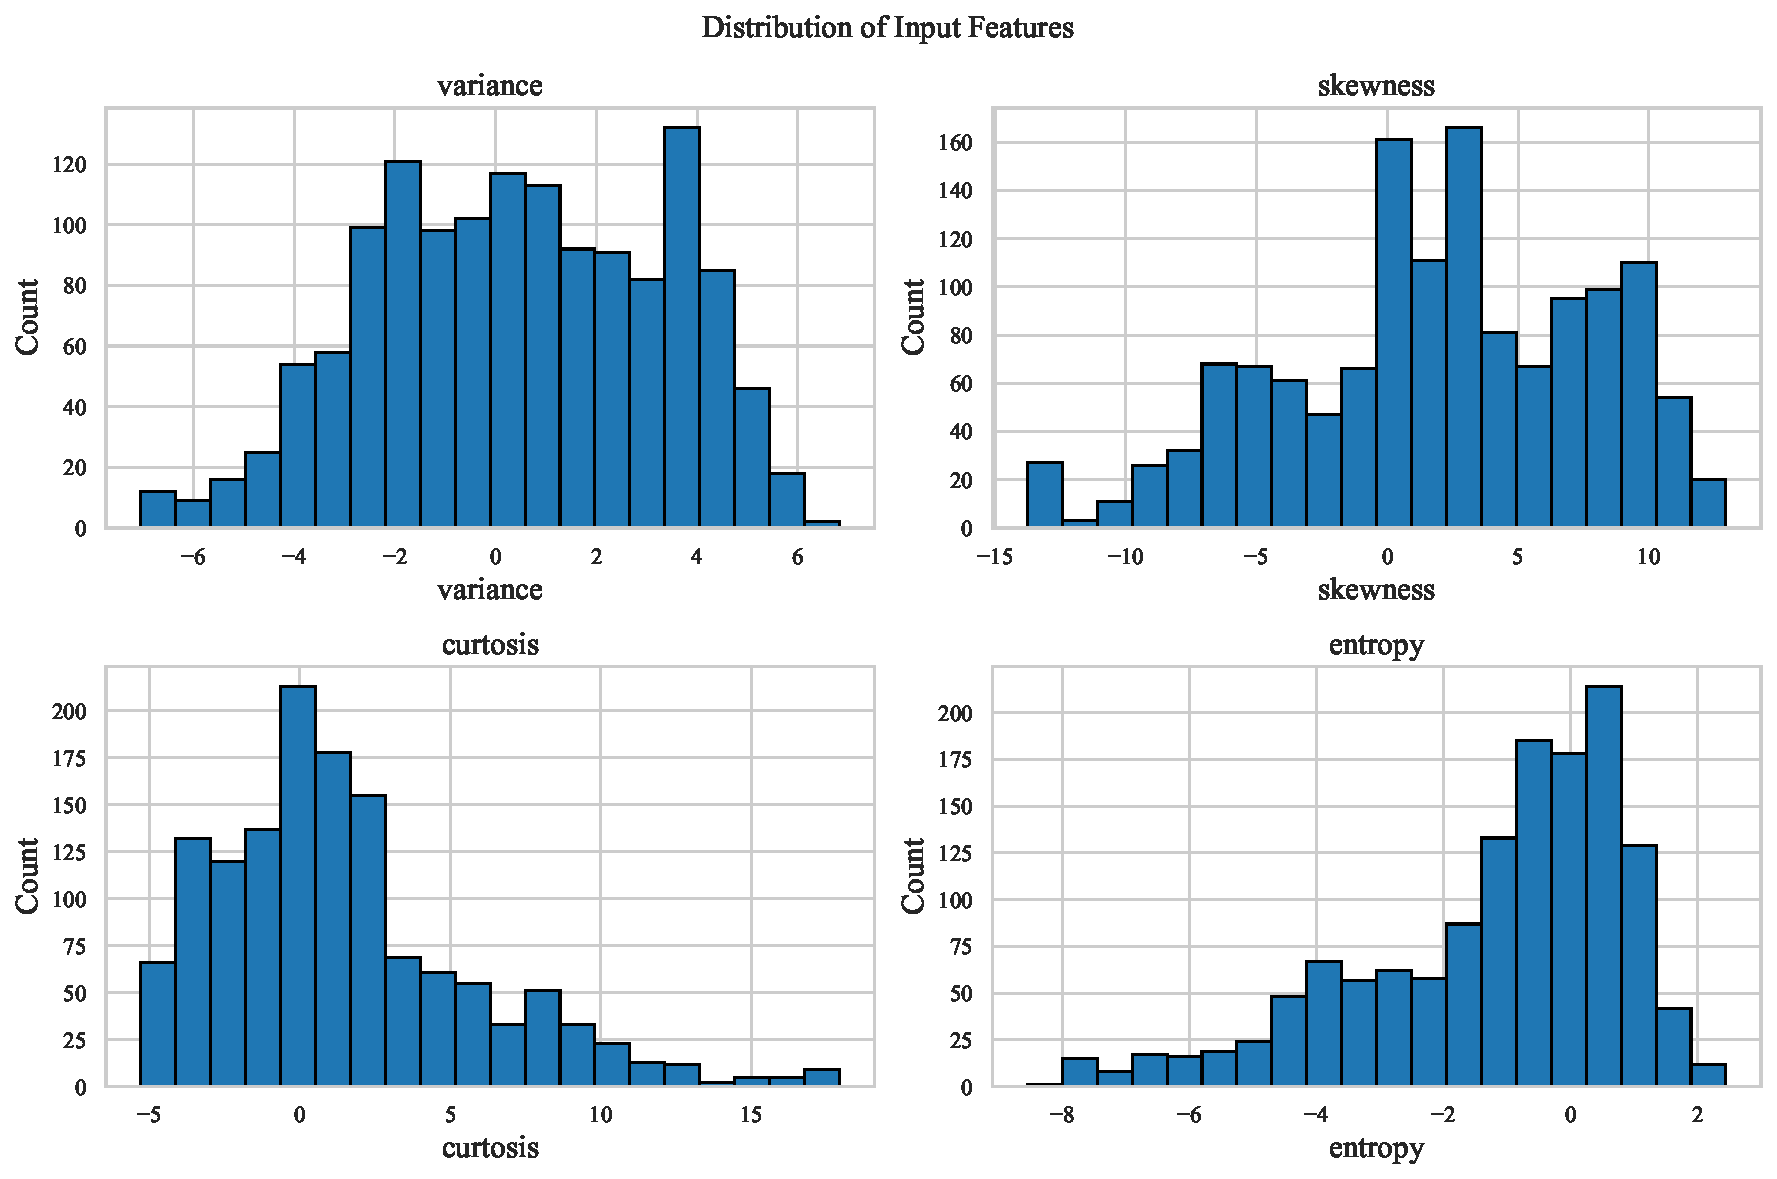
\includegraphics[width=0.85\textwidth]{histograms.pdf}
\caption{Feature Histograms}
\end{figure}
\textbf{Observation:} Variance and Entropy look fairly spread out and close to bell-shaped, while Skewness and Curtosis have a longer tail on the right with a few extreme values -- a sign the raw features aren't on a comparable scale, which is exactly why standardizing them later matters.

\begin{figure}[H]
\centering
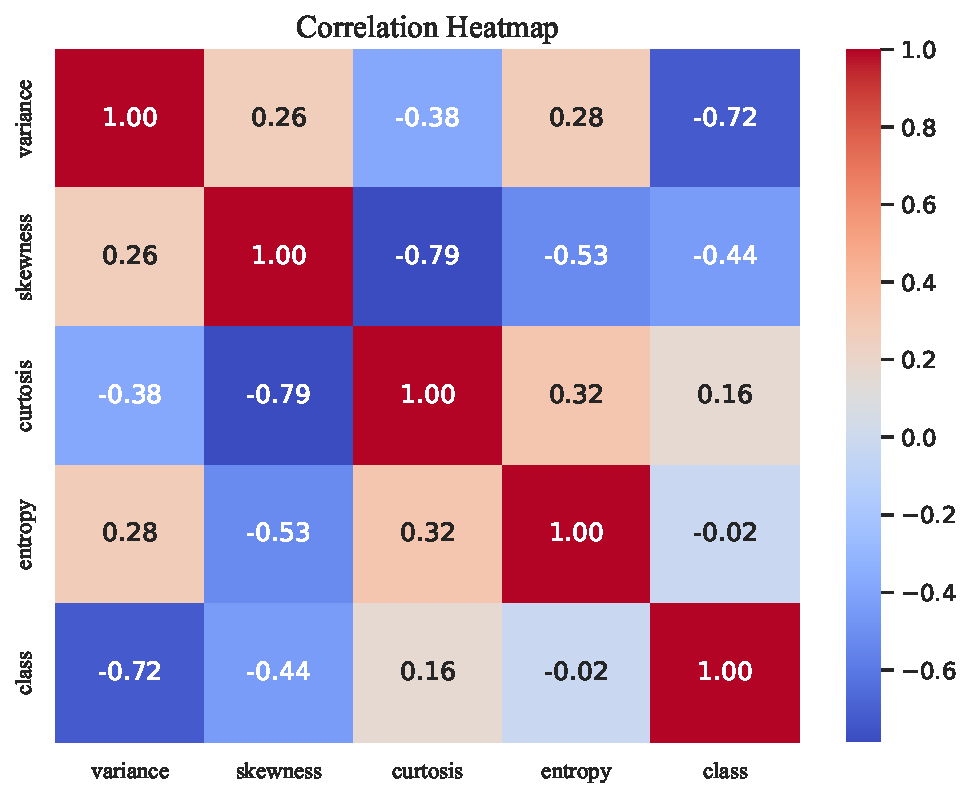
\includegraphics[width=0.6\textwidth]{correlation_heatmap.pdf}
\caption{Correlation Heatmap}
\end{figure}
\textbf{Observation:} Variance has the strongest (negative) correlation with the class label, with Skewness close behind -- these two features are doing most of the work for classification. Skewness and Curtosis are also correlated with each other, which makes sense since both describe the shape of the same underlying image distribution.

\begin{figure}[H]
\centering
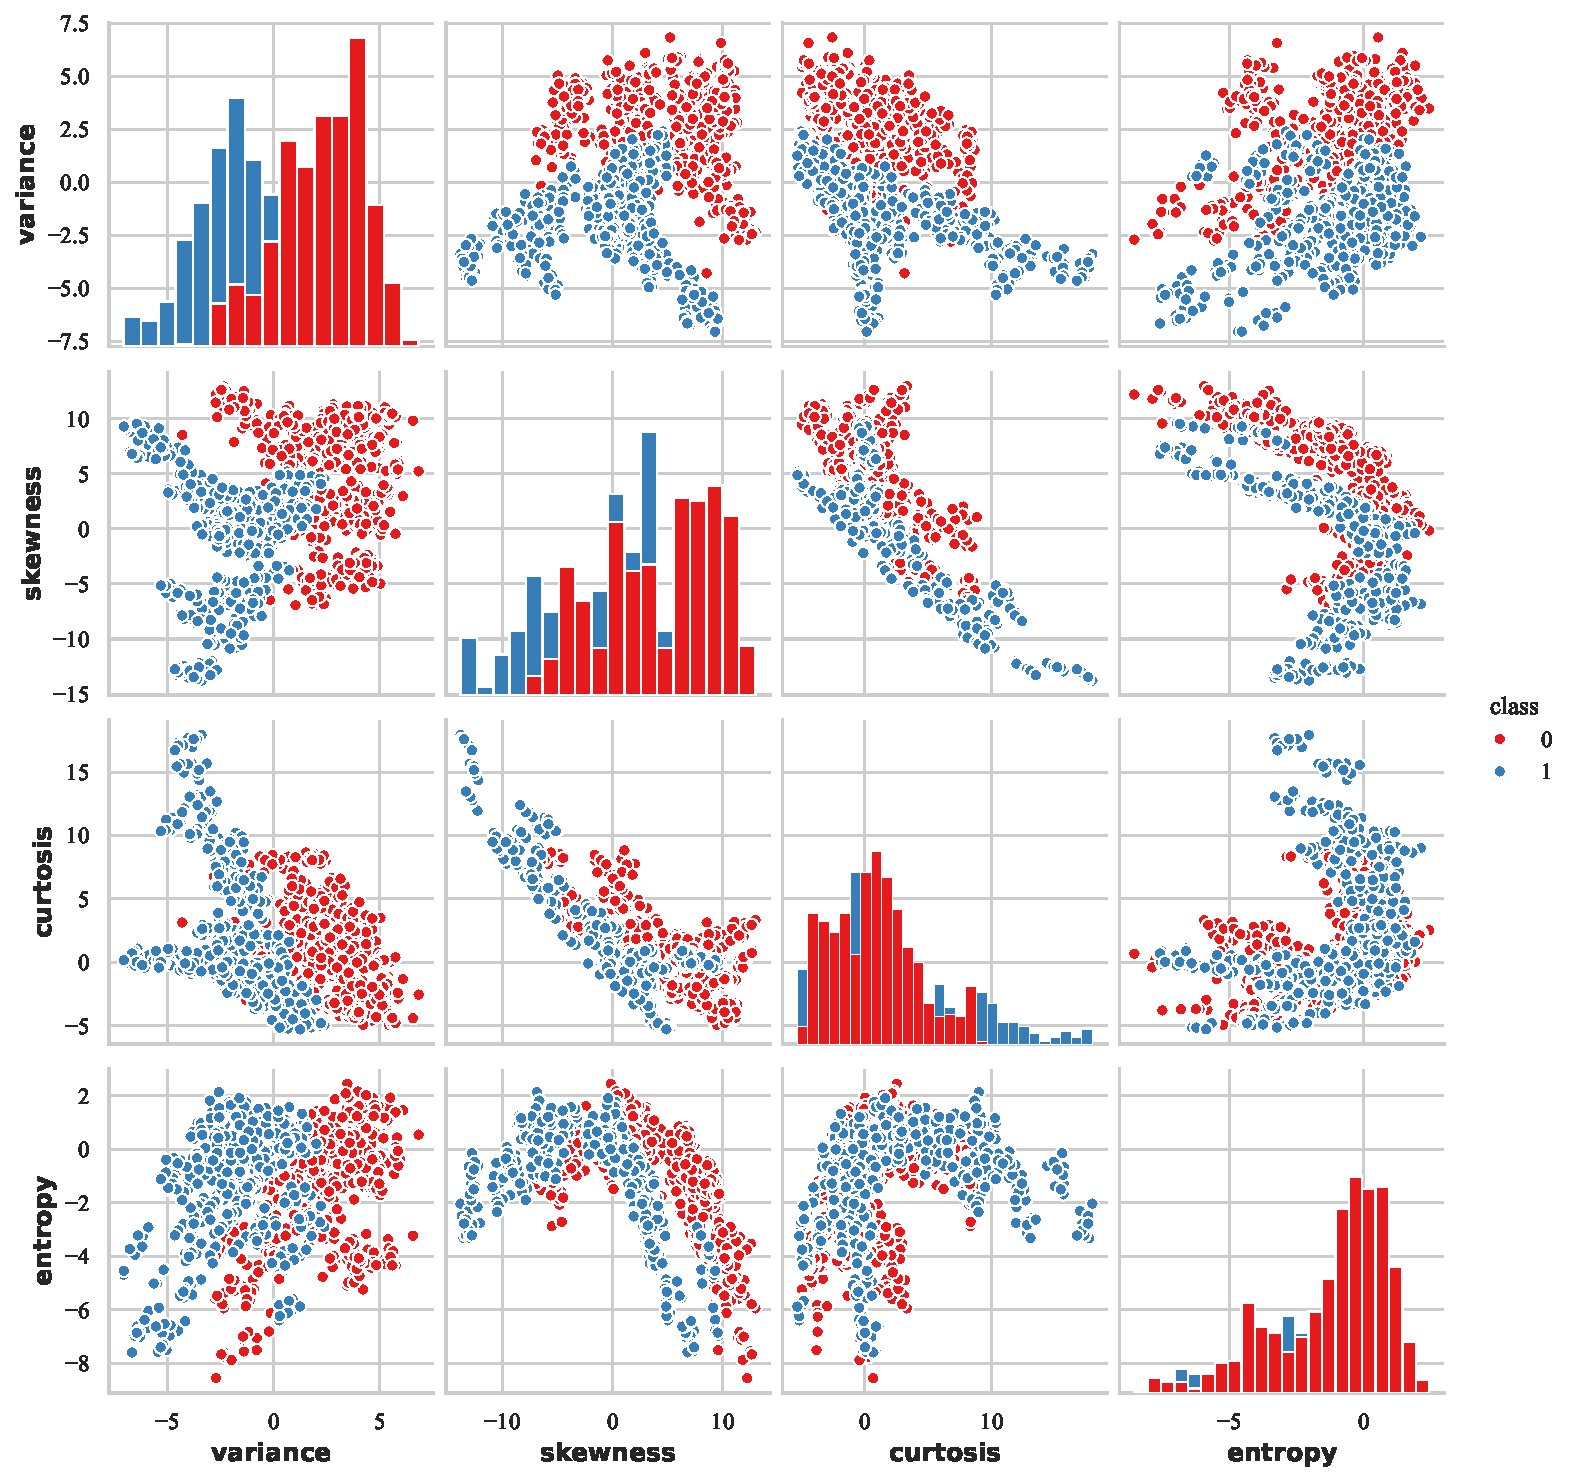
\includegraphics[width=0.9\textwidth]{scatter_plot.pdf}
\caption{Pairwise Scatter Plot Matrix, Coloured by Class}
\end{figure}
\textbf{Observation:} Across every pair of features, the two classes form mostly separate clusters, especially along Variance and Skewness, with only a bit of overlap -- an early sign that a linear model like the perceptron should work well here.

\begin{figure}[H]
\centering
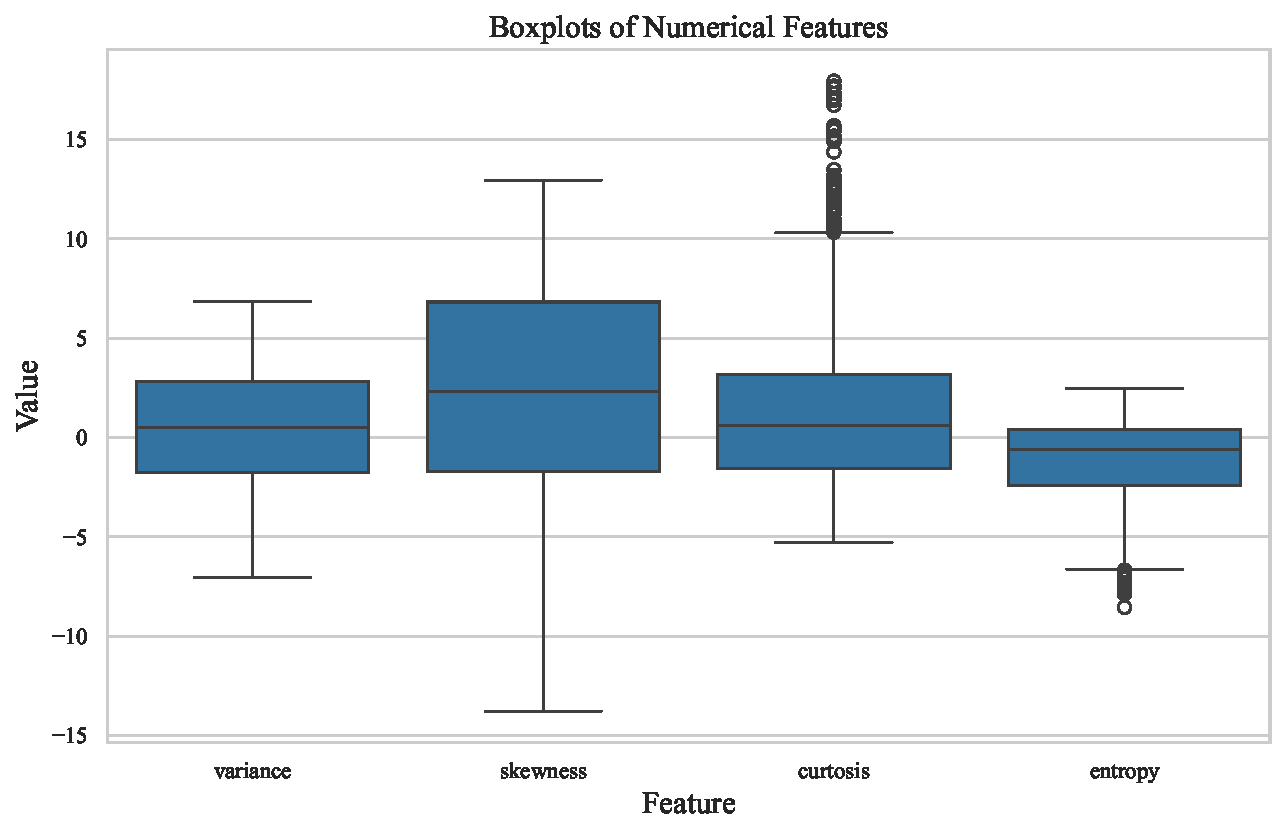
\includegraphics[width=0.85\textwidth]{boxplots.pdf}
\caption{Boxplots of Features}
\end{figure}
\textbf{Observation:} Skewness and Curtosis have a fair number of outlier points beyond the whiskers, while Variance and Entropy are more tightly contained -- another point in favour of standardizing before training.

\begin{figure}[H]
\centering
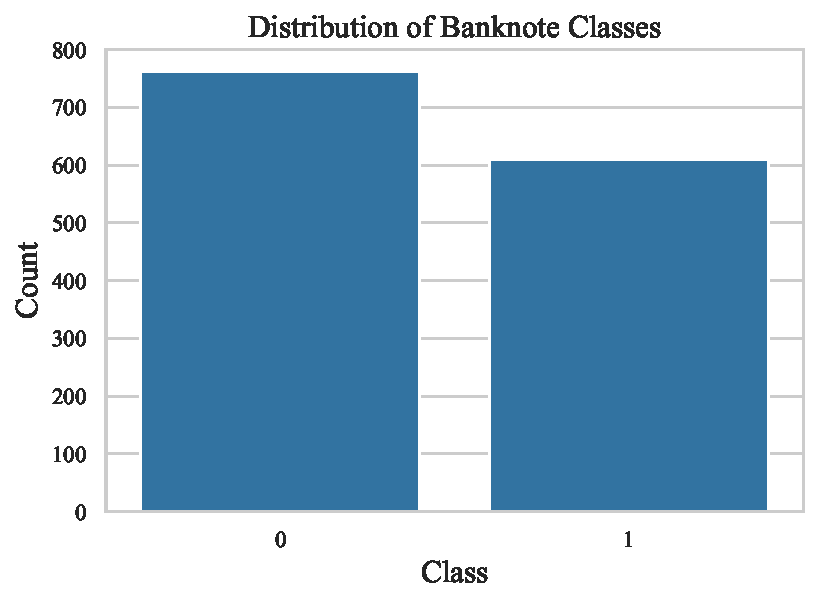
\includegraphics[width=0.5\textwidth]{class_distribution.pdf}
\caption{Class Distribution}
\end{figure}
\textbf{Observation:} The class split (55.5\% vs. 44.5\%) is close enough to balanced that no class-imbalance handling was needed for this experiment.

\begin{figure}[H]
\centering
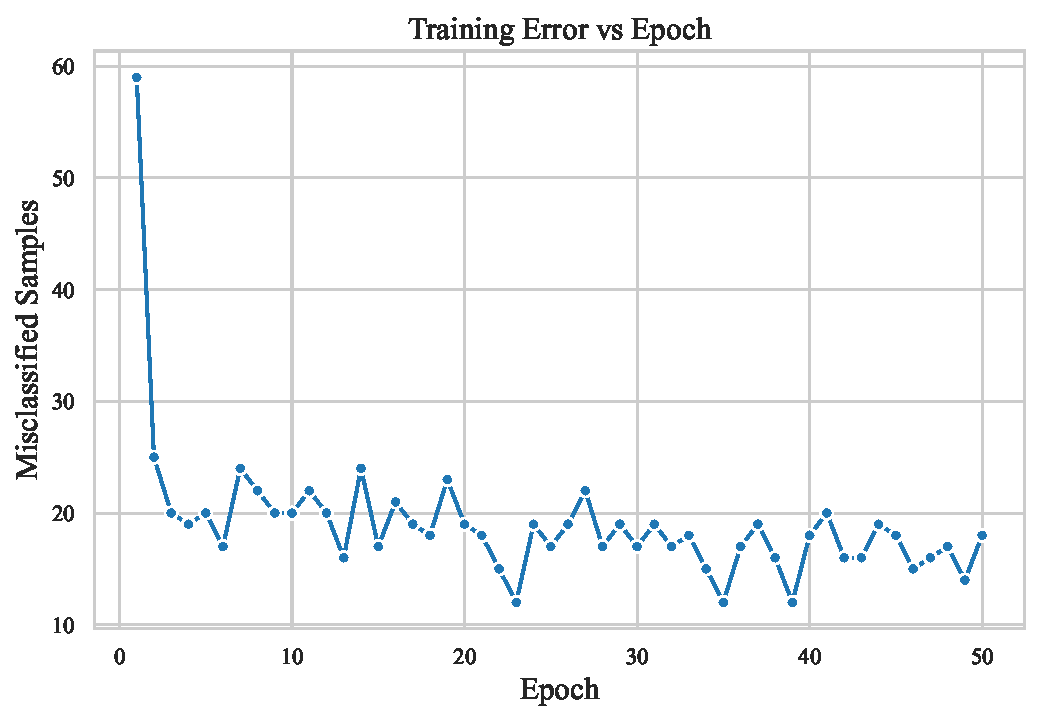
\includegraphics[width=0.6\textwidth]{training_error_vs_epoch.pdf}
\caption{Training Error vs. Epoch}
\end{figure}
\textbf{Observation:} The error drops fast, from 59 down to about 20, within the first handful of epochs, and then hovers between roughly 12 and 24 for the rest of training, never quite reaching zero since the classes overlap slightly.

\begin{figure}[H]
\centering
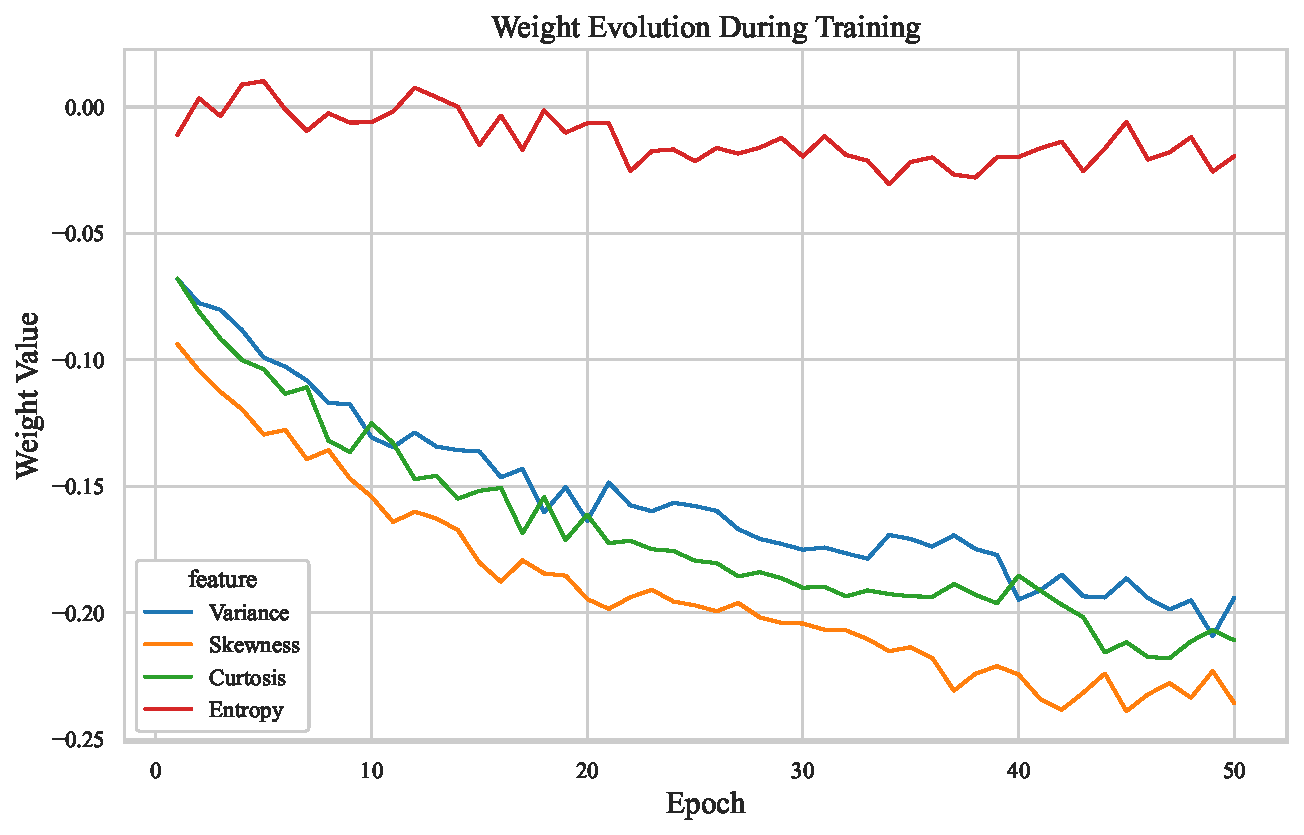
\includegraphics[width=0.6\textwidth]{weight_evolution.pdf}
\caption{Weight Evolution over Epochs}
\end{figure}
\textbf{Observation:} All four weights move quickly away from zero early on and then settle. Variance, Skewness and Curtosis end up with the largest weights, while Entropy stays close to zero throughout, matching what the correlation heatmap already suggested.

\begin{figure}[H]
\centering
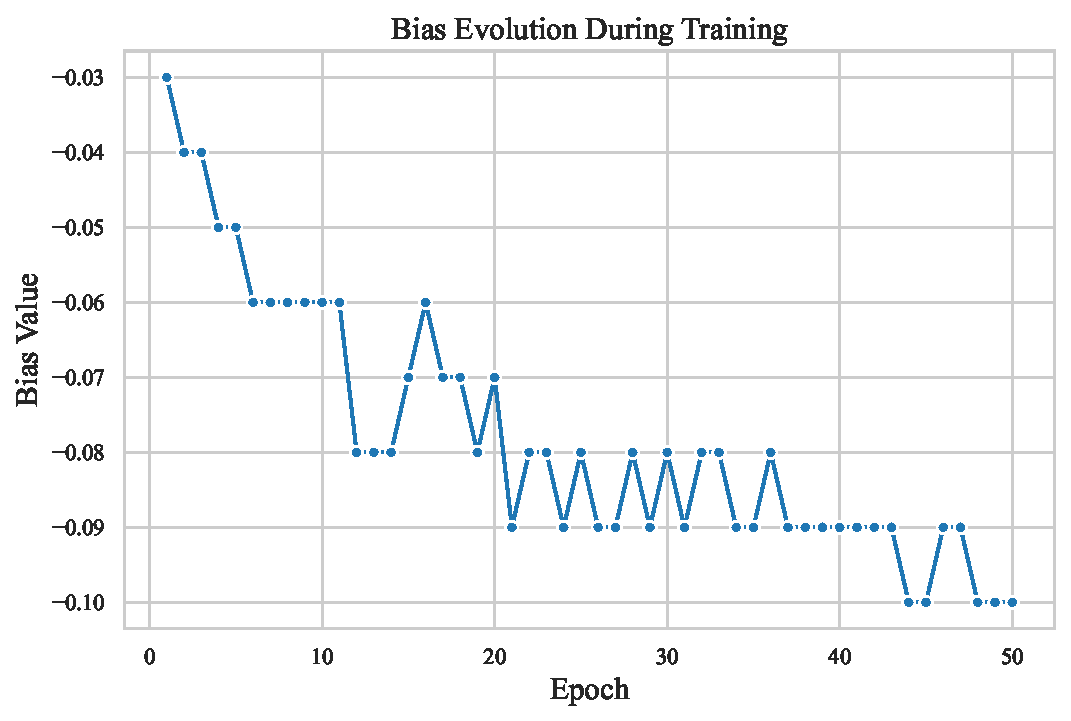
\includegraphics[width=0.6\textwidth]{bias_evolution.pdf}
\caption{Bias Evolution over Epochs}
\end{figure}
\textbf{Observation:} The bias steadily drifts more negative and settles around $-0.10$, shifting the decision boundary away from the origin to better fit the data.

\begin{figure}[H]
\centering
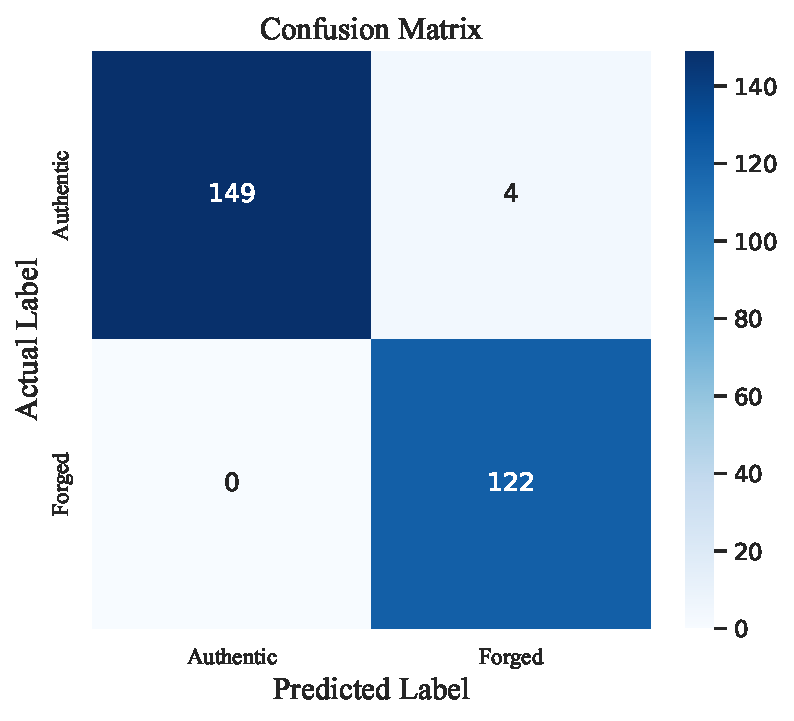
\includegraphics[width=0.5\textwidth]{confusion_matrix.pdf}
\caption{Confusion Matrix}
\end{figure}
\textbf{Observation:} 149 authentic and 122 forged notes were classified correctly, with only 4 false positives and zero false negatives -- the model never let a forged note through undetected.

\begin{figure}[H]
\centering
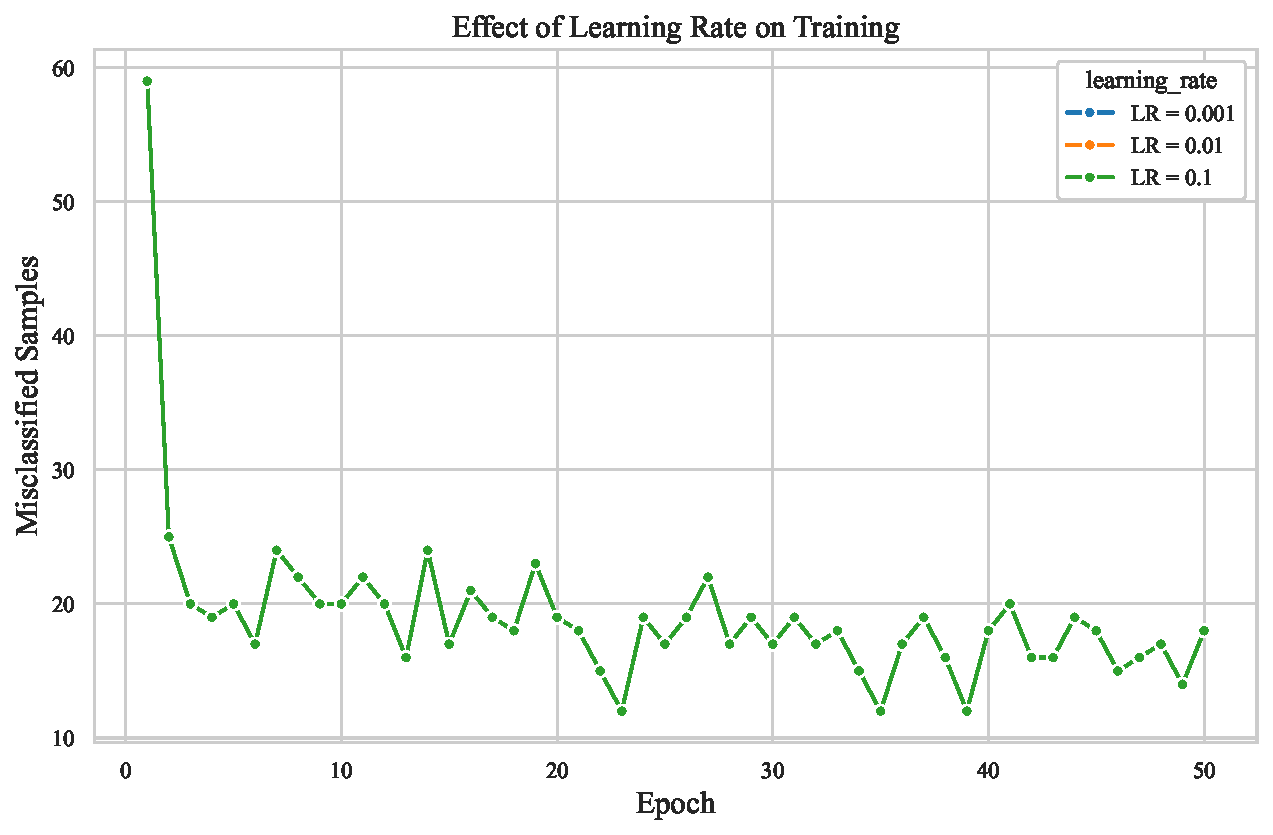
\includegraphics[width=0.6\textwidth]{learning_rate_comparison.pdf}
\caption{Learning Rate Comparison}
\end{figure}
\textbf{Observation:} All three learning rates reach the same final accuracy, but the internal error trajectory is visibly more erratic at the highest rate (0.1) and much smoother at the lowest (0.001).

\begin{figure}[H]
\centering
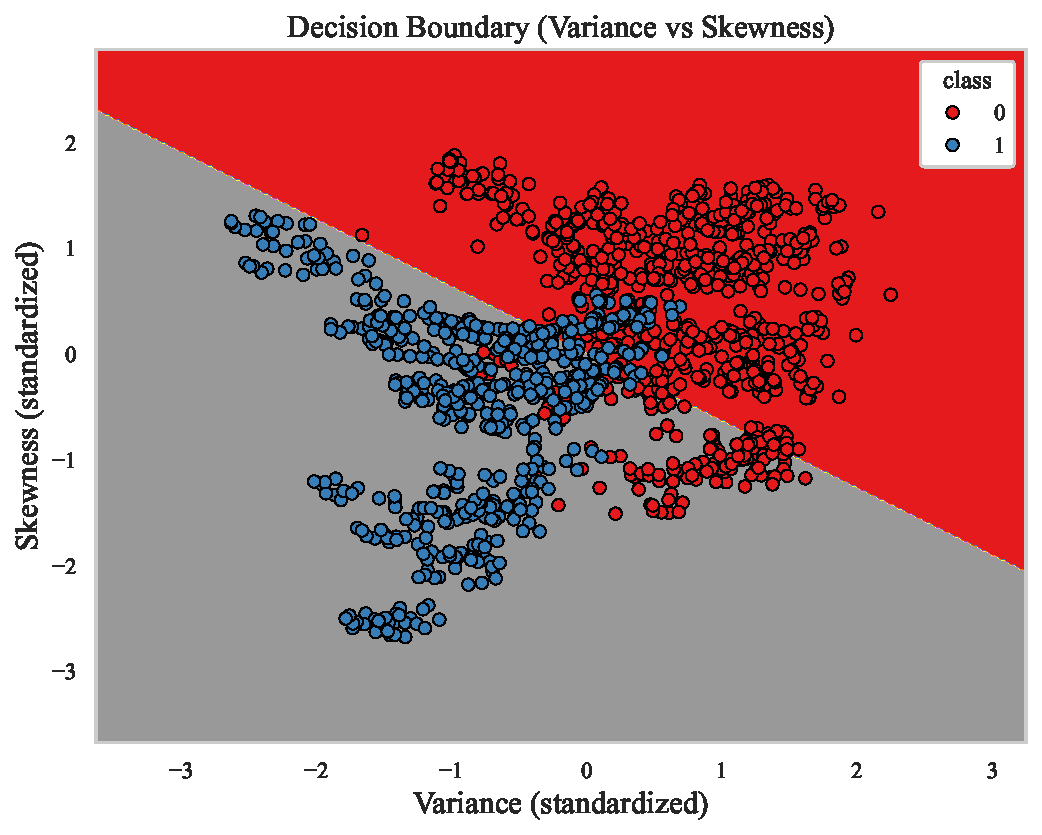
\includegraphics[width=0.6\textwidth]{decision_boundary.pdf}
\caption{Decision Boundary using Variance and Skewness}
\end{figure}
\textbf{Observation:} The 2D boundary still separates most of the two classes reasonably well, but the visible overlap region is wider than it would be with all four features available.

\begin{figure}[H]
\centering
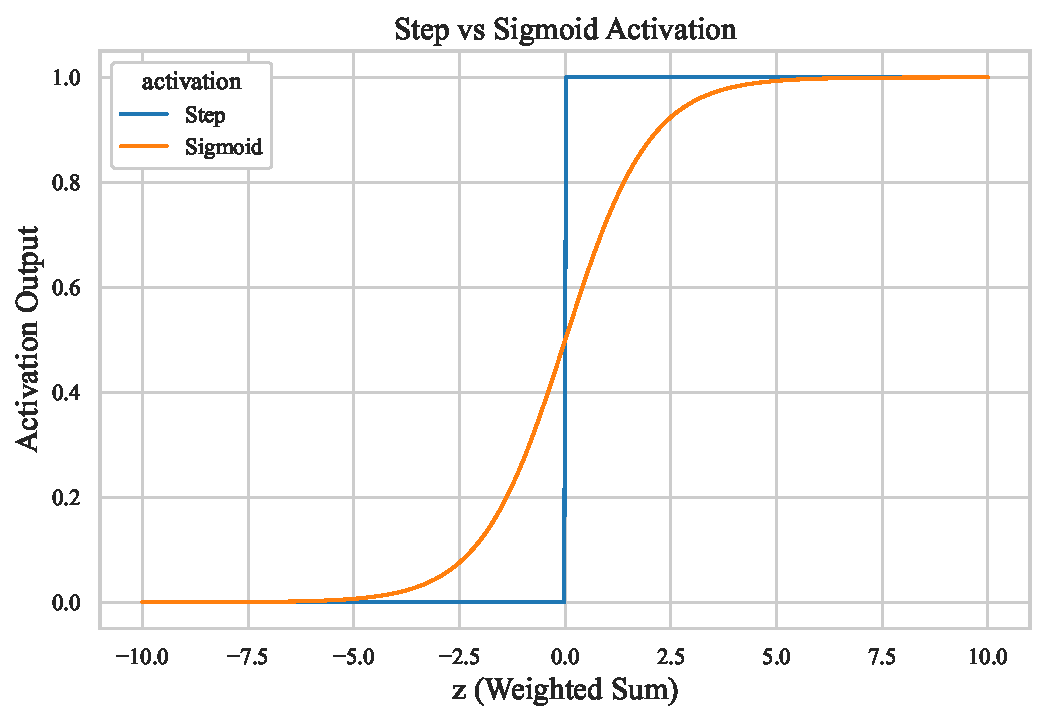
\includegraphics[width=0.6\textwidth]{step_vs_sigmoid_comparison.pdf}
\caption{Step vs. Sigmoid Activation}
\end{figure}
\textbf{Observation:} The Step function jumps sharply between 0 and 1 with no usable slope anywhere, while the Sigmoid curve is smooth and differentiable across its entire range -- exactly the property that makes gradient-based training possible.

\begin{figure}[H]
\centering
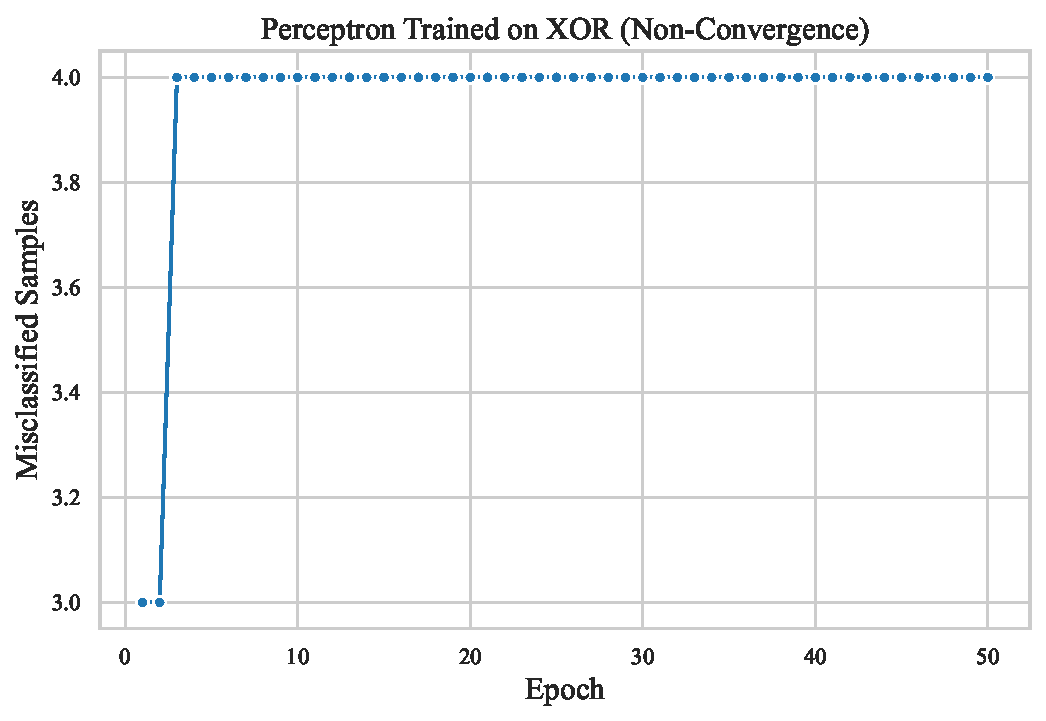
\includegraphics[width=0.6\textwidth]{xor_limitation_demo.pdf}
\caption{Perceptron Trained on XOR -- Non-Convergence}
\end{figure}
\textbf{Observation:} The error never drops to zero and stays flat near 3--4 misclassifications out of 4 points for the entire run -- direct experimental proof that a single straight-line boundary cannot solve XOR.

\begin{figure}[H]
\centering
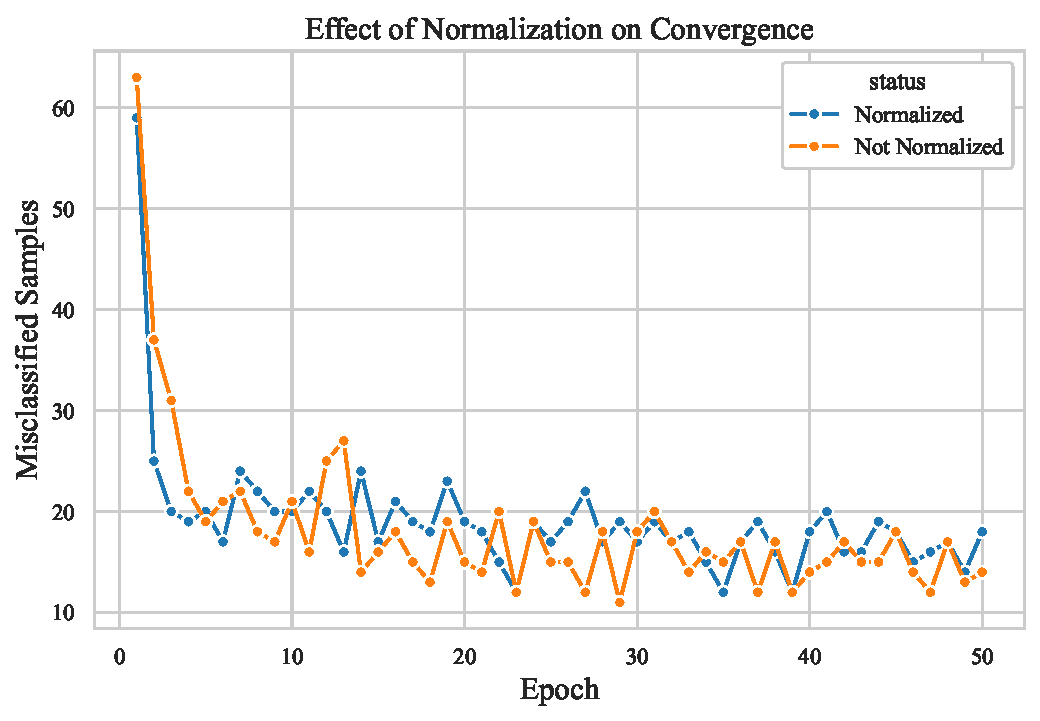
\includegraphics[width=0.6\textwidth]{normalization_effect_comparison.pdf}
\caption{Effect of Normalization on Convergence}
\end{figure}
\textbf{Observation:} The normalized run's error curve is both lower overall and noticeably smoother than the raw-feature run's curve, making the benefit of standardization clearly visible.

%----------------------------------------------------------

\section*{9. Performance Tables}

\begin{table}[H]
\centering
\caption{Training Summary}
\begin{tabular}{ll}
\toprule
Dataset Size & 1372 \\
Train/Test Split & 1097 / 275 (80\% / 20\%, stratified) \\
Learning Rate & 0.01 \\
Epochs & 50 \\
Final Weights & $[-0.1941,\ -0.2358,\ -0.2109,\ -0.0195]$ \\
Final Bias & $-0.1000$ \\
Accuracy & 0.9855 \\
Precision & 0.9683 \\
Recall & 1.0000 \\
F1-score & 0.9839 \\
\bottomrule
\end{tabular}
\end{table}

\begin{table}[H]
\centering
\caption{Epoch-wise Learning (Selected Epochs)}
\begin{tabular}{cccccc}
\toprule
Epoch & Errors & Weight 1 (Variance) & Weight 2 (Skewness) & Weight 3 (Curtosis) & Bias\\
\midrule
1  & 59 & -0.0680 & -0.0938 & -0.0678 & -0.0300 \\
5  & 20 & -0.0991 & -0.1295 & -0.1037 & -0.0500 \\
10 & 20 & -0.1307 & -0.1541 & -0.1250 & -0.0600 \\
20 & 19 & -0.1636 & -0.1946 & -0.1613 & -0.0700 \\
30 & 17 & -0.1751 & -0.2043 & -0.1901 & -0.0800 \\
40 & 18 & -0.1948 & -0.2244 & -0.1853 & -0.0900 \\
50 & 18 & -0.1941 & -0.2358 & -0.2109 & -0.1000 \\
\bottomrule
\end{tabular}
\end{table}

%----------------------------------------------------------

\section*{10. Discussion}

This experiment provides a clear, practical demonstration of how a perceptron learns, beyond the theoretical formulation alone. The model reached 98.55\% accuracy with perfect recall on the test set, consistent with the EDA pairplot, which suggested the dataset is close to linearly separable -- explaining why a simple linear model such as the perceptron performs well on it.

Several observations are worth highlighting:

\begin{itemize}[leftmargin=*]
\item The learning rate had little effect on \textit{final} accuracy in this case, but it clearly changed \textit{how} the model reached that point -- larger learning rates cause much larger, more erratic swings in the weights and bias during training.
\item Cross-checking against Scikit-learn's own Perceptron served as a useful validation step, confirming that the from-scratch implementation was not producing results by coincidence -- the two models performed almost identically.
\item Reducing the feature set to two dimensions for the decision-boundary plot noticeably degraded performance, indicating that even features with small final weights (such as Entropy) contribute meaningfully in combination with the others.
\item The XOR experiment made the linear-separability limitation directly observable rather than purely theoretical -- the error remained permanently stuck, providing concrete evidence of the boundary this class of model cannot cross.
\item The Step activation function is the central limitation of this approach: it can only express straight-line decision boundaries, provides no confidence or probability estimate, and yields no gradient signal at all. This is precisely why it is replaced by smooth, differentiable activations such as Sigmoid and ReLU in deeper, multilayer networks.
\end{itemize}

%----------------------------------------------------------

\section*{11. Conclusion}

\begin{itemize}[leftmargin=*]
\item Built a Single Layer Perceptron completely from scratch in NumPy and trained it on the real-world Banknote Authentication dataset.
\item Achieved \textbf{98.55\% accuracy}, \textbf{96.83\% precision}, \textbf{100\% recall}, and a \textbf{98.39\% F1-score} on the held-out test set.
\item Validated the implementation against Scikit-learn's Perceptron, which scored a close \textbf{97.82\% accuracy} -- confirming the from-scratch model was implemented correctly.
\item Learning rate (0.001 / 0.01 / 0.1) changed the training dynamics but not the final accuracy on this dataset.
\item Feature normalization made a real, visible difference to how smoothly and reliably the model converged.
\item Demonstrated experimentally that a single-layer perceptron cannot solve the XOR problem, since XOR is not linearly separable -- this is the exact reason Multilayer Perceptrons exist.
\item Overall, this experiment built a solid, practical foundation for the deeper architectures coming up later in this course, since every one of them is ultimately built out of these same basic ideas: weights, biases, activation functions, and gradient-based learning.
\end{itemize}

%----------------------------------------------------------

\section*{12. References}

\begin{enumerate}
\item F. Rosenblatt, ``The Perceptron,'' \emph{Psychological Review}, 1958.
\item I. Goodfellow, Y. Bengio and A. Courville, \emph{Deep Learning}, MIT Press, 2016.
\item C. M. Bishop, \emph{Pattern Recognition and Machine Learning}, Springer, 2006.
\item S. Haykin, \emph{Neural Networks and Learning Machines}, Pearson, 2009.
\item UCI Machine Learning Repository -- Banknote Authentication Dataset.
\item Scikit-learn Documentation: Perceptron.
\end{enumerate}

\end{document}\documentclass[11pt]{article}
\usepackage[margin=1in]{geometry}
\usepackage{amsmath,amssymb,booktabs,array,longtable}
\usepackage{graphicx}
\graphicspath{{figures/}}
\usepackage{hyperref}
\usepackage{enumitem}
\usepackage{titlesec}
\usepackage{float}
\usepackage{caption}
\usepackage{mathtools}
\usepackage{setspace}

\onehalfspacing

\begin{document}

\begin{center}
{\LARGE\textbf{Shiv Nadar University Chennai}}\\[4mm]
\end{center}

\renewcommand{\arraystretch}{1.6}
\setlength{\tabcolsep}{10pt}

\begin{center}
\begin{tabular}{|p{4cm}|p{9.5cm}|}
\hline
\textbf{Degree \& Branch} & B.Tech Artificial Intelligence \& Data Science, Semester V \\ \hline
\textbf{Subject} & CS3807 -- Deep Learning Laboratory \\ \hline
\textbf{Name} & Madhav.S \\ \hline
\textbf{Section} & AIDS `B' \\ \hline
\textbf{Register Number} & 24011101066 \\ \hline
\end{tabular}
\end{center}

\vspace{5mm}

\begin{center}
{\Large\textbf{Experiment 1}}\\[1mm]
{\large\textbf{Implementation of a Single Layer Perceptron for Binary Classification}}
\end{center}

\vspace{4mm}

%----------------------------------------------------------

\section*{1. Objective}

The goal of this experiment is to understand how a single artificial neuron works and to build a Single Layer Perceptron completely from scratch, without relying on any deep learning library, so that the underlying learning process is fully visible. The experiment aims to build familiarity with the perceptron learning rule, demonstrate why activation functions matter, visualize the model's learning progress epoch by epoch, and evaluate its performance on a real-world dataset rather than a synthetic example.

%----------------------------------------------------------

\section*{2. Background Theory}

An \textbf{artificial neuron} is the basic computing unit of a neural network. It takes in one or more input features, multiplies each of them by a weight, adds a bias term, and then passes the result through an activation function to produce an output.

The \textbf{Single Layer Perceptron} is the oldest and simplest of these models. It can only learn to separate two classes when they are (roughly) linearly separable, i.e., when a single straight line or flat plane can divide the data into its two classes.

\subsection*{Mathematical Formulation}

\textbf{Weighted Sum} -- every input is combined into a single number $z$:

\[
z=\mathbf{w}^{T}\mathbf{x}+b
\]

where

\begin{itemize}
\item $\mathbf{x}$ is the input vector (the feature values of one sample),
\item $\mathbf{w}$ is the weight vector (how much importance each feature gets),
\item $b$ is the bias (shifts the decision boundary away from the origin),
\item $z$ is the resulting linear combination.
\end{itemize}

\textbf{Prediction} -- the weighted sum is passed through an activation function $f$:

\[
\hat y=f(z)
\]

\textbf{Weight Update Rule} -- after every wrong prediction, the weights are nudged in the direction that would have made the prediction correct:

\[
\mathbf{w}_{new}
=
\mathbf{w}_{old}
+
\eta
(y-\hat y)
\mathbf{x}
\]

\textbf{Bias Update} -- the bias is updated the same way:

\[
b_{new}
=
b_{old}
+
\eta
(y-\hat y)
\]

Here $\eta$ (eta) is the \textbf{learning rate} -- it controls how big a step is taken at each update.

%----------------------------------------------------------

\section*{3. Activation Functions}

An activation function decides what a neuron actually outputs once it has computed its weighted sum. Without it, a neural network -- no matter how many layers it has -- would behave like a single linear equation, since stacking linear operations just gives another linear operation. Activation functions are what let networks learn curved, complex decision boundaries.

\subsection*{Step Activation Function}

This experiment uses only the step function, since that is what the classical perceptron uses:

\[
f(z)=
\begin{cases}
1,&z\ge0\\
0,&z<0
\end{cases}
\]

It simply outputs 1 or 0 depending on which side of zero $z$ falls on. Because of this hard cutoff, it can only ever draw a straight decision boundary, and it cannot be used for anything more advanced than basic linear classification.

\begin{table}[H]
\centering
\caption{Common Activation Functions}
\begin{tabular}{lll}
\toprule
\textbf{Activation} & \textbf{Output Range} & \textbf{Typically Used In} \\
\midrule
Step        & $\{0,1\}$          & Classical Perceptron \\
Sigmoid     & $(0,1)$            & Binary classification output layers \\
Tanh        & $(-1,1)$           & Hidden layers of older-style networks \\
ReLU        & $[0,\infty)$       & Hidden layers of CNNs and MLPs \\
Leaky ReLU  & $(-\infty,\infty)$ & Avoiding the ``dying ReLU'' problem \\
Softmax     & $(0,1)$            & Multi-class classification output layers \\
\bottomrule
\end{tabular}
\end{table}

\textit{Note: only the Step function is used here. The rest will come up in later experiments once we move to Multilayer Perceptrons.}

%----------------------------------------------------------

\section*{4. Dataset Description}

\textbf{Dataset:} Banknote Authentication Dataset\\
\textbf{Source:} UCI Machine Learning Repository, fetched directly in code via the \texttt{ucimlrepo} package (\texttt{id=267})\\
\textbf{Link:} \url{https://archive.ics.uci.edu/dataset/267/banknote+authentication}

\begin{table}[H]
\centering
\caption{Dataset Summary}
\begin{tabular}{ll}
\toprule
Instances & 1372 \\
Features & 4 numerical features \\
Classes & 2 \\
Missing Values & None \\
Task & Binary classification \\
\bottomrule
\end{tabular}
\end{table}

The four features come from applying a wavelet transform to images of genuine and forged banknotes:

\begin{itemize}
\item Variance
\item Skewness
\item Curtosis
\item Entropy
\end{itemize}

Target Class:

\begin{itemize}
\item 0 -- Authentic Banknote
\item 1 -- Forged Banknote
\end{itemize}

The classes are reasonably balanced: 762 authentic notes (55.5\%) and 610 forged notes (44.5\%), so accuracy alone is still a fairly trustworthy metric here.

%----------------------------------------------------------

\section*{5. Experimental Procedure}

\textbf{Task 1 -- Dataset Exploration:} The dataset was loaded using \texttt{fetch\_ucirepo(id=267)}, and the features and target were combined into a single DataFrame. Its shape, missing values, and descriptive statistics were examined before any further processing.

\textbf{Task 2 -- Exploratory Data Analysis:} Feature histograms, a correlation heatmap, a pairwise scatter plot matrix, and boxplots were generated to understand the shape, spread, and relationships of the four features, along with a class-distribution plot to check class balance.

\textbf{Task 3 -- Data Preprocessing:} All four features were standardized to zero mean and unit variance using \texttt{StandardScaler}, and the data was split into 80\% training and 20\% testing using stratified sampling so both sets preserve the same class ratio.

\textbf{Task 4 -- Perceptron Implementation:} The perceptron was implemented entirely from scratch in NumPy -- weight and bias initialization, the step activation function, forward propagation, and the perceptron learning rule -- without using any machine learning library for this part.

\textbf{Task 5 -- Model Training:} The perceptron was trained for 50 epochs with a learning rate of $\eta = 0.01$, logging the epoch number, number of misclassified samples, and the updated weights and bias after every epoch.

\textbf{Task 6 -- Model Evaluation:} The trained model was evaluated on the held-out test set using accuracy, precision, recall, F1-score, and a confusion matrix.

\textbf{Task 7 -- Learning Rate Study:} Training was repeated from scratch with three different learning rates (0.001, 0.01, 0.1) to observe how the choice of $\eta$ affects convergence behaviour.

\textbf{Task 8 -- Comparison with Scikit-learn (Optional):} \texttt{sklearn.linear\_model.Perceptron} was trained on the same train/test split, and its metrics were compared against the from-scratch implementation as a validation step.

In addition to the eight core tasks, five additional tasks were carried out: comparing the Step and Sigmoid activation functions, the Scikit-learn comparison above, the learning-rate study above, an experimental demonstration of why a single-layer perceptron cannot solve the XOR problem, and a study of how feature normalization affects convergence speed and stability.

%----------------------------------------------------------

\section*{6. Source Code}

The complete implementation, exactly as run in Colab, is hosted on GitHub rather than reproduced in full here, so that the report stays readable and the code stays easy to browse, run, and update independently:

\begin{center}
\url{https://github.com/<your-username>/<your-repo-name>}
\end{center}

The repository contains the full notebook (\texttt{notebook/deep\_learning\_lab\_1.ipynb}), the exported script (\texttt{src/deep\_learning\_lab\_1\_final.py}), the \texttt{requirements.txt} needed to run it, and this report's LaTeX source.

%----------------------------------------------------------

\section*{7. Experimental Results}

\subsection*{Dataset Summary}

\begin{table}[H]
\centering
\caption{Descriptive Statistics of the Dataset}
\begin{tabular}{lrrrr}
\toprule
 & Variance & Skewness & Curtosis & Entropy \\
\midrule
mean & 0.4337 & 1.9224 & 1.3976 & -1.1917 \\
std  & 2.8428 & 5.8690 & 4.3100 & 2.1010 \\
min  & -7.0421 & -13.7731 & -5.2861 & -8.5482 \\
25\% & -1.7730 & -1.7082 & -1.5750 & -2.4135 \\
50\% & 0.4962 & 2.3197 & 0.6166 & -0.5867 \\
75\% & 2.8215 & 6.8146 & 3.1793 & 0.3948 \\
max  & 6.8248 & 12.9516 & 17.9274 & 2.4495 \\
\bottomrule
\end{tabular}
\end{table}

No missing values were found in any column. After preprocessing, the split produced \textbf{1097 training samples} and \textbf{275 testing samples}.

\subsection*{Training Outcome}

The perceptron was trained for 50 epochs at $\eta = 0.01$. Misclassifications fell sharply from 59 to about 20 within the first few epochs, then fluctuated between roughly 12 and 24 for the remainder of training without reaching zero -- expected behaviour, since the two classes overlap slightly and are not perfectly linearly separable. A sample of the training log:

\begin{verbatim}
Epoch  1 | Errors:  59 | Bias: -0.0300 | Weights: [-0.0680 -0.0938 -0.0678 -0.0110]
Epoch  5 | Errors:  20 | Bias: -0.0500 | Weights: [-0.0991 -0.1295 -0.1037  0.0102]
Epoch 10 | Errors:  20 | Bias: -0.0600 | Weights: [-0.1307 -0.1541 -0.1250 -0.0060]
Epoch 20 | Errors:  19 | Bias: -0.0700 | Weights: [-0.1636 -0.1946 -0.1613 -0.0064]
Epoch 30 | Errors:  17 | Bias: -0.0800 | Weights: [-0.1751 -0.2043 -0.1901 -0.0196]
Epoch 40 | Errors:  18 | Bias: -0.0900 | Weights: [-0.1948 -0.2244 -0.1853 -0.0197]
Epoch 50 | Errors:  18 | Bias: -0.1000 | Weights: [-0.1941 -0.2358 -0.2109 -0.0195]
\end{verbatim}

The full epoch-wise log is summarized in Section 9, Performance Tables.

\subsection*{Test Set Evaluation}

\begin{table}[H]
\centering
\caption{Test Set Performance of the Scratch Perceptron (LR = 0.01, 50 epochs)}
\begin{tabular}{lc}
\toprule
Metric & Value \\
\midrule
Accuracy & 0.9855 \\
Precision & 0.9683 \\
Recall & 1.0000 \\
F1-score & 0.9839 \\
\bottomrule
\end{tabular}
\end{table}

Out of 275 test samples, 149 authentic notes and 122 forged notes were correctly classified. Only 4 authentic notes were wrongly flagged as forged, and \textbf{not a single forged note was missed} (0 false negatives) -- a significant result in a fraud-detection context, where failing to flag a forged note is a far costlier error than being overly cautious about a genuine one.

\subsection*{Learning Rate Study}

\begin{table}[H]
\centering
\caption{Effect of Learning Rate on Test Performance}
\begin{tabular}{lcc}
\toprule
Learning Rate & Accuracy & Epochs Run \\
\midrule
0.001 & 0.9855 & 50 \\
0.01  & 0.9855 & 50 \\
0.1   & 0.9855 & 50 \\
\bottomrule
\end{tabular}
\end{table}

All three learning rates reached the same final test accuracy, and none converged to zero training error within 50 epochs. A larger learning rate (0.1) causes much larger swings in the weights and bias at every update, while a smaller rate (0.001) updates far more cautiously -- both still explored a similar enough region of weight space to land on comparably good decision boundaries.

\subsection*{Comparison with Scikit-learn}

\begin{table}[H]
\centering
\caption{Scratch Implementation vs. Scikit-learn's Perceptron}
\begin{tabular}{lcccc}
\toprule
Model & Accuracy & Precision & Recall & F1-score \\
\midrule
Scratch Perceptron & 0.9855 & 0.9683 & 1.0000 & 0.9839 \\
Scikit-learn Perceptron & 0.9782 & 0.9677 & 0.9836 & 0.9756 \\
\bottomrule
\end{tabular}
\end{table}

Both implementations perform well, with the from-scratch model slightly ahead on recall and F1-score -- confirmation that the manually implemented update rule was correct and consistent with the standard algorithm.

\subsection*{Decision Boundary (Optional)}

Retraining using only two features (Variance and Skewness) for the sake of a 2D visualization resulted in a much higher training error -- around 190 out of 1097 samples, roughly 17\% -- with little improvement over 50 epochs. This indicates that the remaining two features contribute meaningfully to separability in the full four-feature model.

\subsection*{Why a Single Layer Perceptron Cannot Solve XOR}

XOR is not linearly separable: the points $(0,0)$ and $(1,1)$ belong to class 0, while $(0,1)$ and $(1,0)$ belong to class 1, and no single straight line can separate all the 0s from all the 1s. This was confirmed experimentally -- the perceptron's error never dropped to zero on XOR, remaining stuck at 3--4 misclassifications out of 4 points for the entire run. Since a single-layer perceptron can only express a linear decision boundary, it fundamentally cannot represent XOR -- solving it requires at least one hidden layer (a Multilayer Perceptron).

\subsection*{Effect of Feature Normalization}

Without normalization, a wide-ranging feature such as Skewness (roughly $-13.8$ to $13.0$) dominates the weighted sum and the resulting weight updates. The model trained on raw, unscaled features produced a much larger final bias ($+0.95$ versus $-0.10$) and noisier updates than the normalized version, confirming that standardizing features before training results in faster and more stable convergence.

%----------------------------------------------------------

\section*{8. Generated Plots with Interpretation}

\begin{figure}[H]
\centering
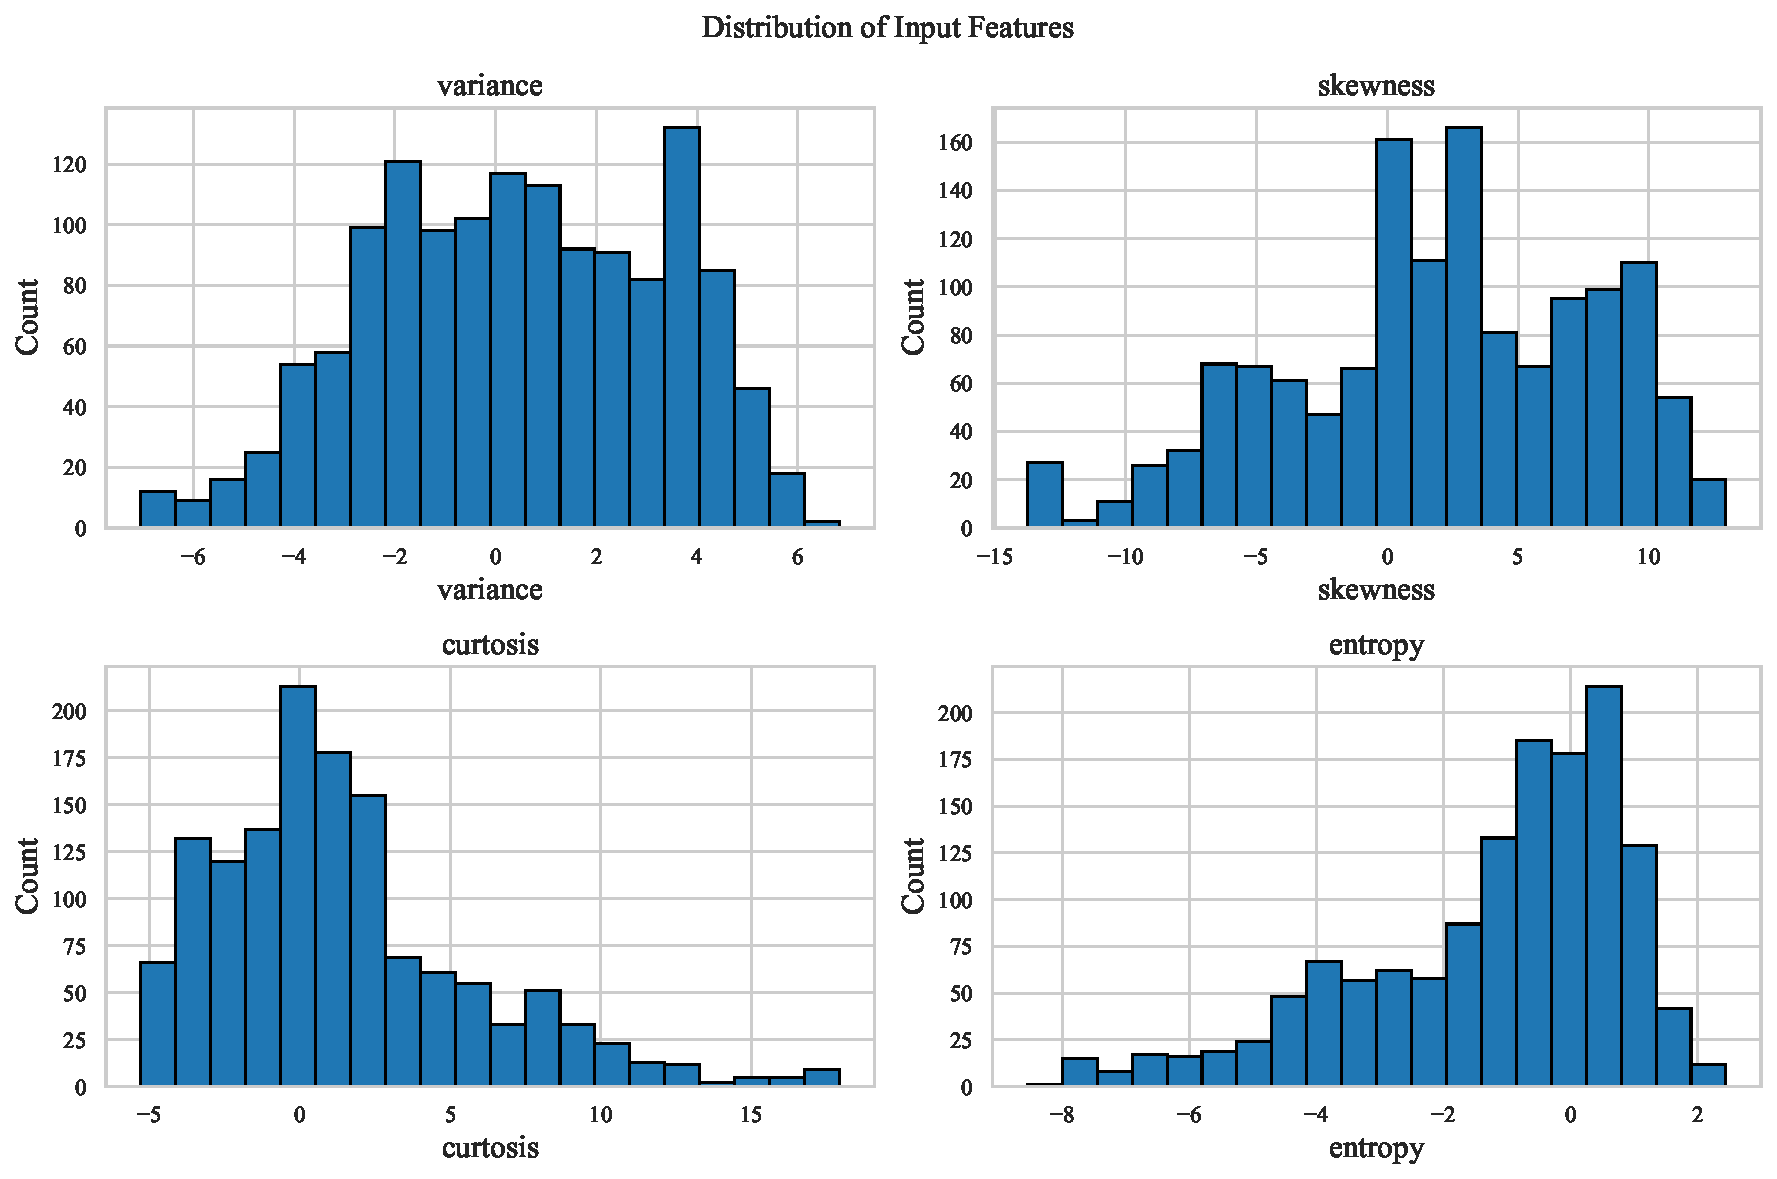
\includegraphics[width=0.85\textwidth]{histograms.pdf}
\caption{Feature Histograms}
\end{figure}
\textbf{Observation:} Variance and Entropy look fairly spread out and close to bell-shaped, while Skewness and Curtosis have a longer tail on the right with a few extreme values -- a sign the raw features aren't on a comparable scale, which is exactly why standardizing them later matters.

\begin{figure}[H]
\centering
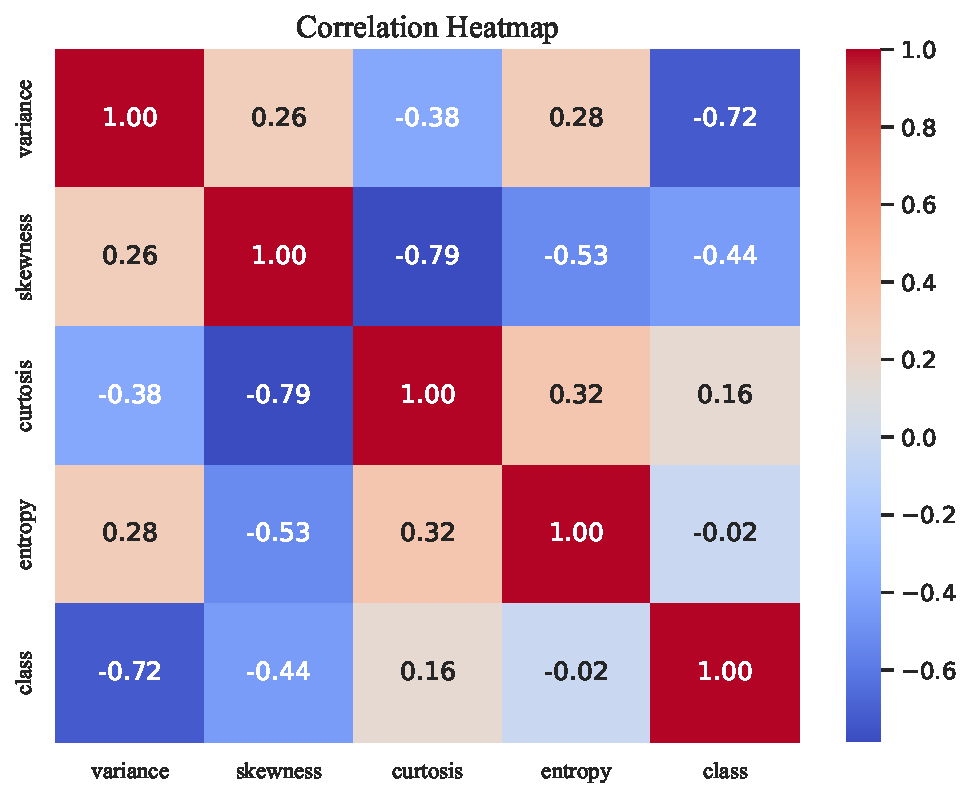
\includegraphics[width=0.6\textwidth]{correlation_heatmap.pdf}
\caption{Correlation Heatmap}
\end{figure}
\textbf{Observation:} Variance has the strongest (negative) correlation with the class label, with Skewness close behind -- these two features are doing most of the work for classification. Skewness and Curtosis are also correlated with each other, which makes sense since both describe the shape of the same underlying image distribution.

\begin{figure}[H]
\centering
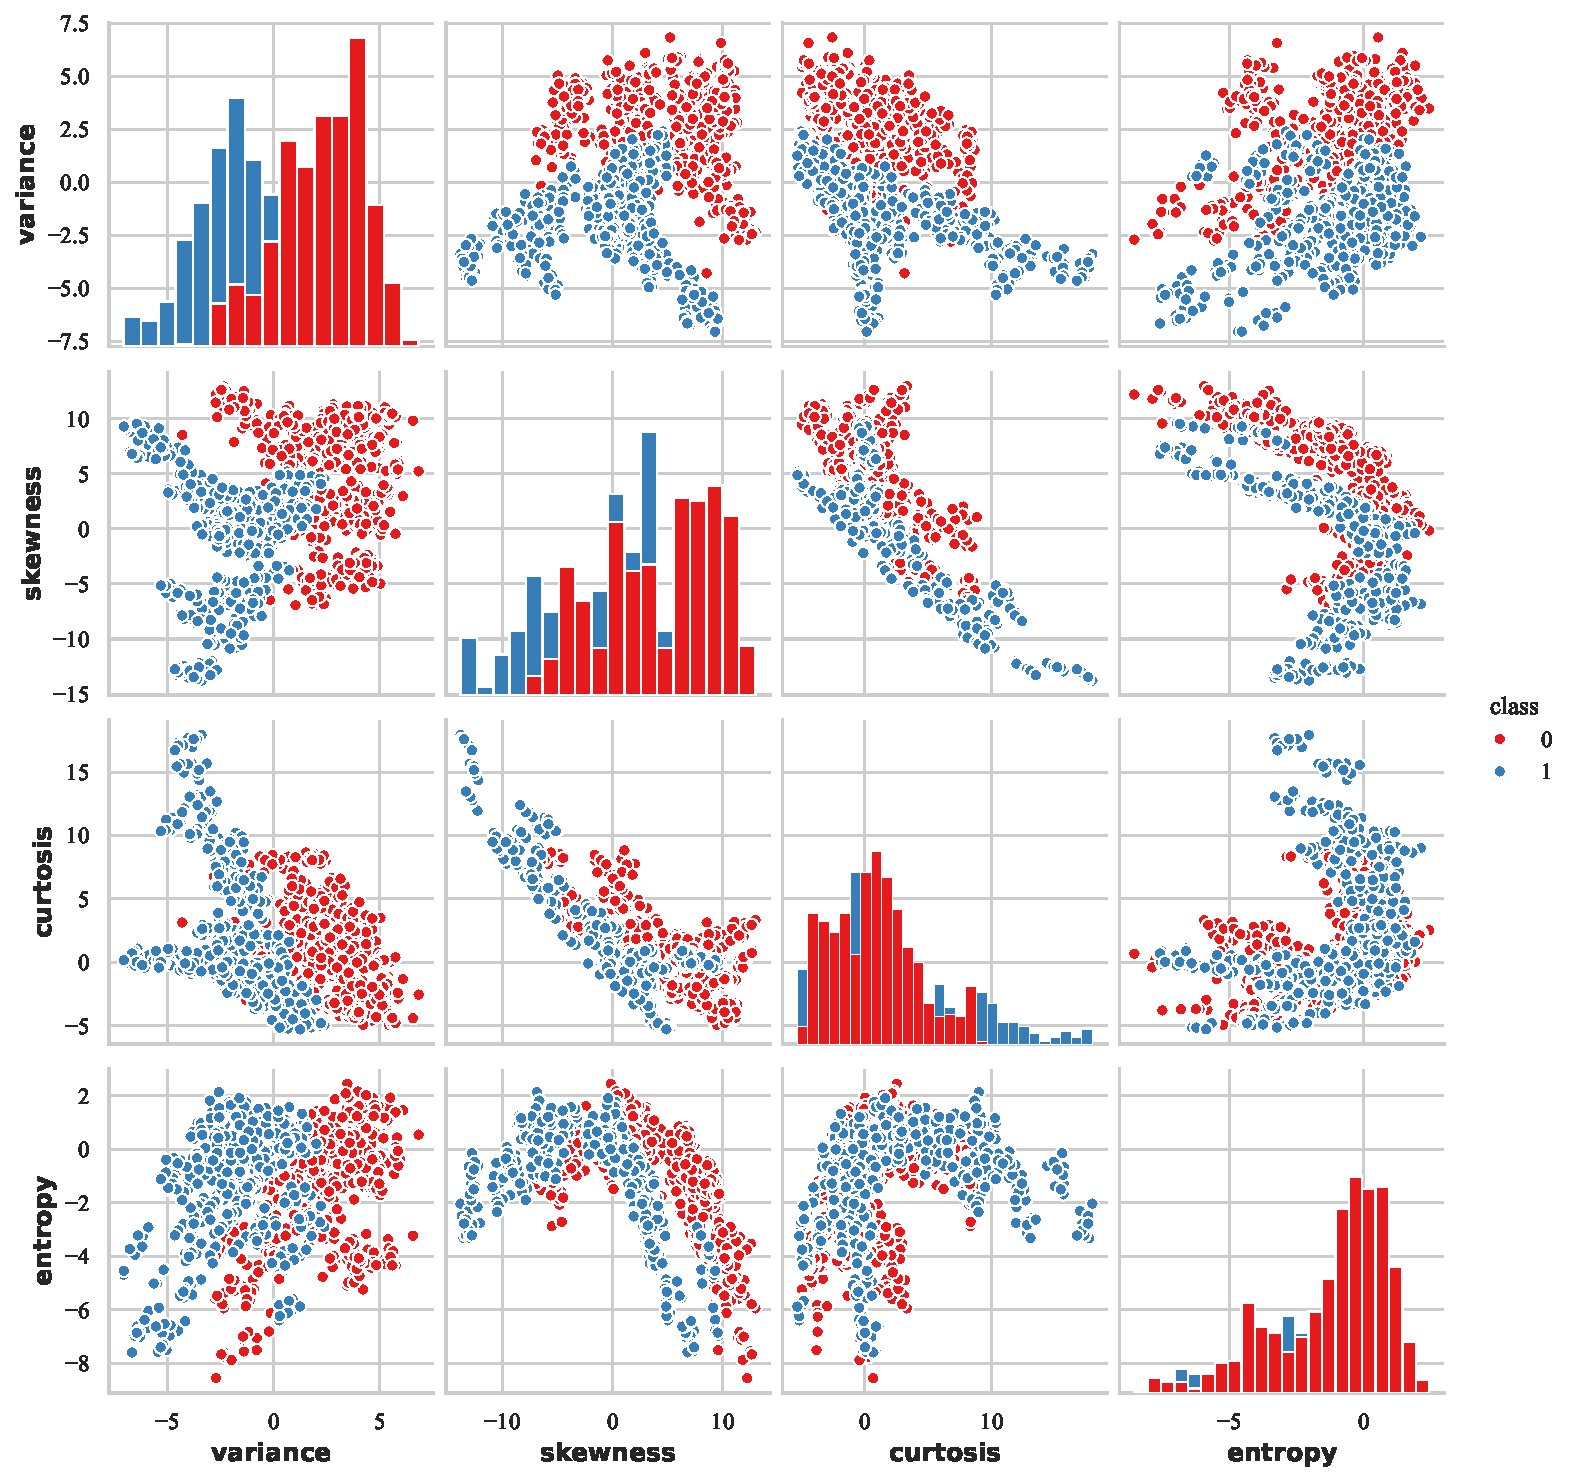
\includegraphics[width=0.9\textwidth]{scatter_plot.pdf}
\caption{Pairwise Scatter Plot Matrix, Coloured by Class}
\end{figure}
\textbf{Observation:} Across every pair of features, the two classes form mostly separate clusters, especially along Variance and Skewness, with only a bit of overlap -- an early sign that a linear model like the perceptron should work well here.

\begin{figure}[H]
\centering
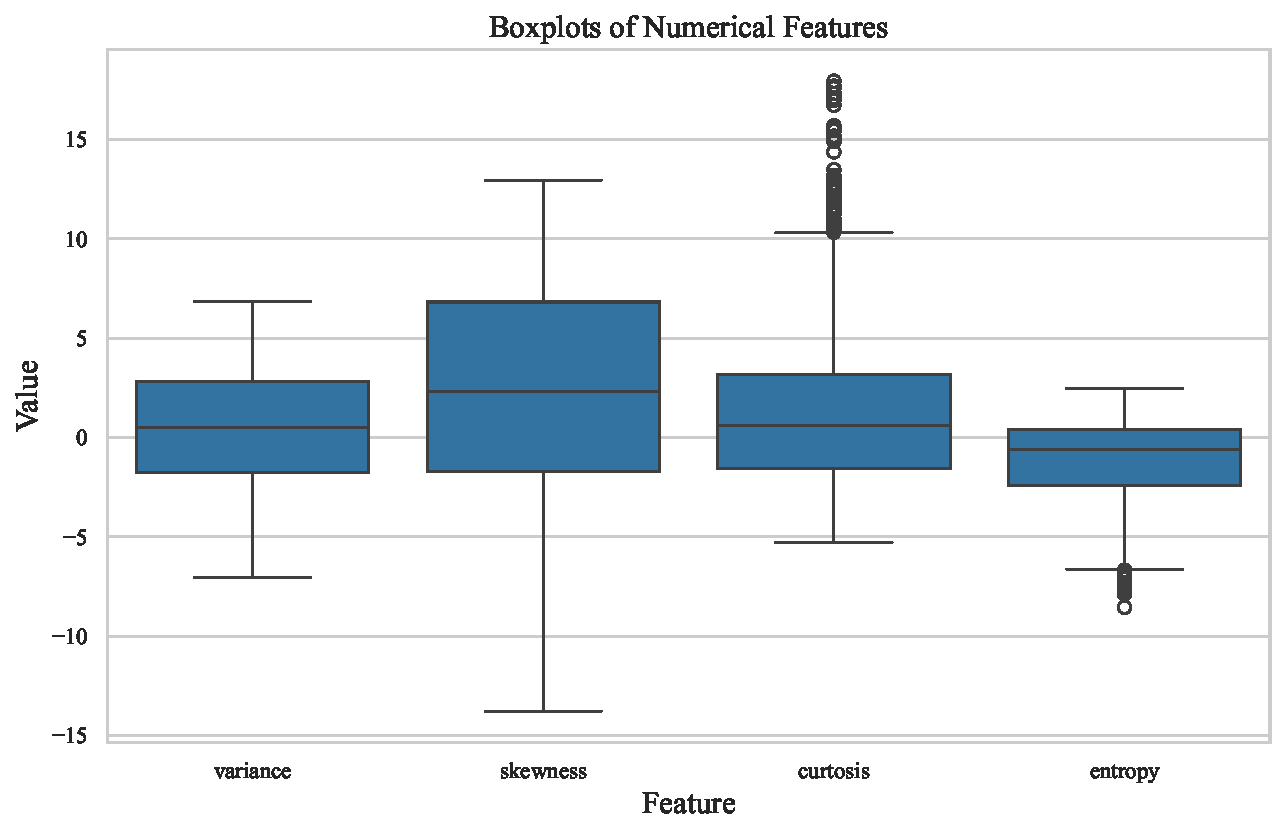
\includegraphics[width=0.85\textwidth]{boxplots.pdf}
\caption{Boxplots of Features}
\end{figure}
\textbf{Observation:} Skewness and Curtosis have a fair number of outlier points beyond the whiskers, while Variance and Entropy are more tightly contained -- another point in favour of standardizing before training.

\begin{figure}[H]
\centering
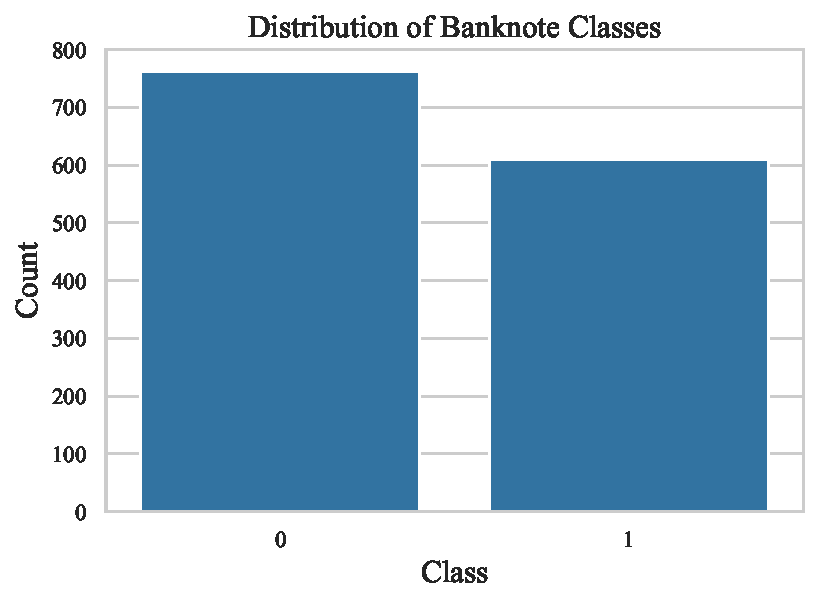
\includegraphics[width=0.5\textwidth]{class_distribution.pdf}
\caption{Class Distribution}
\end{figure}
\textbf{Observation:} The class split (55.5\% vs. 44.5\%) is close enough to balanced that no class-imbalance handling was needed for this experiment.

\begin{figure}[H]
\centering
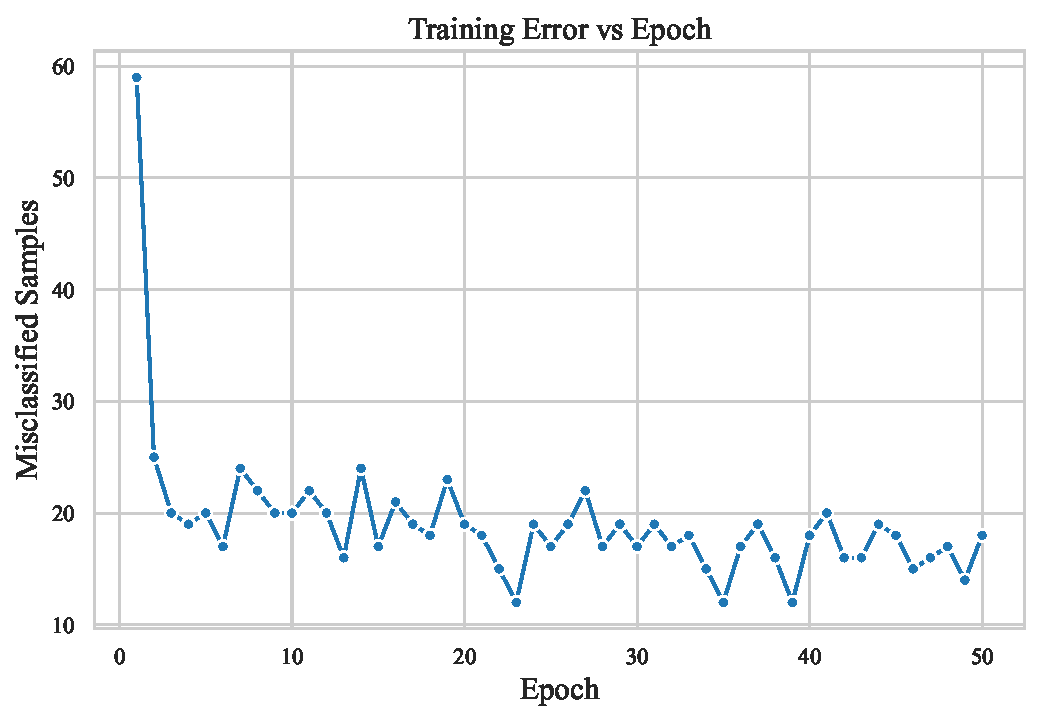
\includegraphics[width=0.6\textwidth]{training_error_vs_epoch.pdf}
\caption{Training Error vs. Epoch}
\end{figure}
\textbf{Observation:} The error drops fast, from 59 down to about 20, within the first handful of epochs, and then hovers between roughly 12 and 24 for the rest of training, never quite reaching zero since the classes overlap slightly.

\begin{figure}[H]
\centering
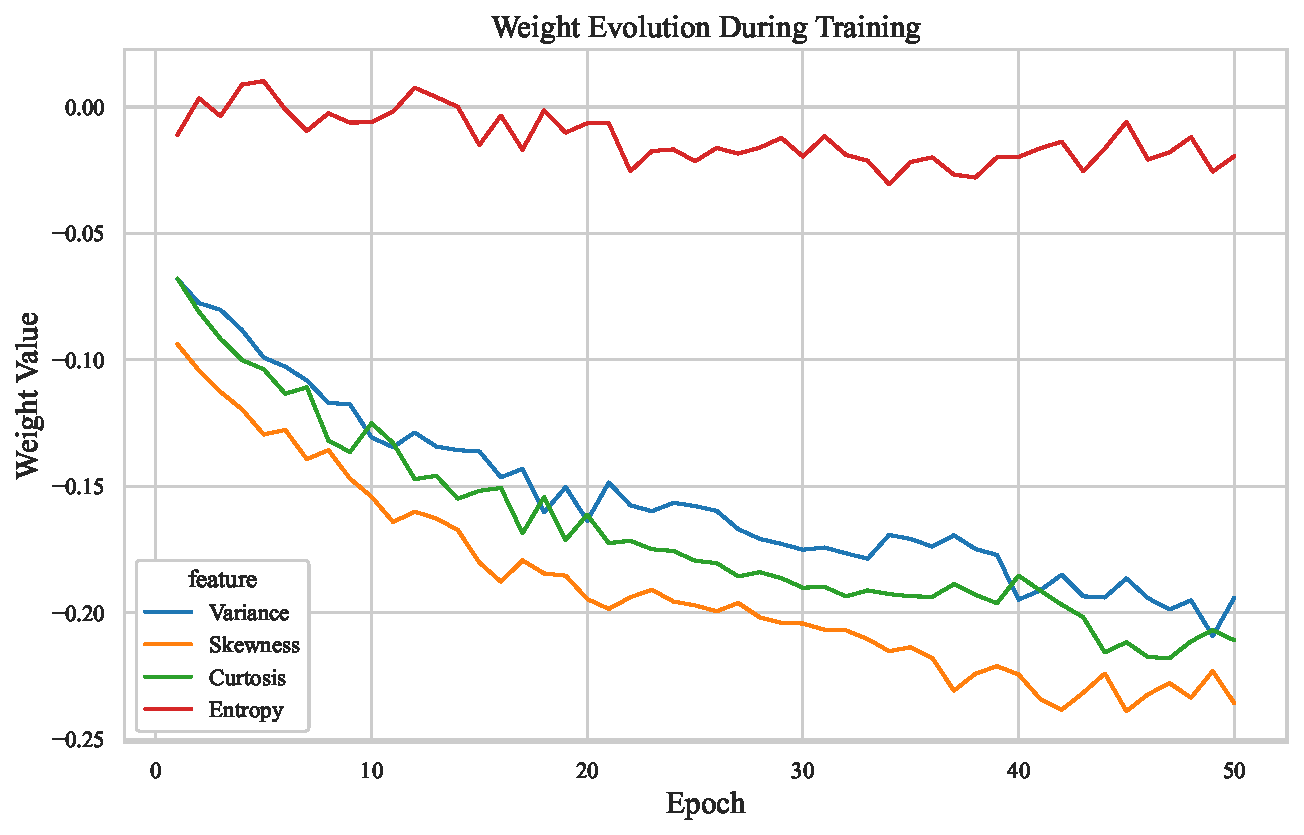
\includegraphics[width=0.6\textwidth]{weight_evolution.pdf}
\caption{Weight Evolution over Epochs}
\end{figure}
\textbf{Observation:} All four weights move quickly away from zero early on and then settle. Variance, Skewness and Curtosis end up with the largest weights, while Entropy stays close to zero throughout, matching what the correlation heatmap already suggested.

\begin{figure}[H]
\centering
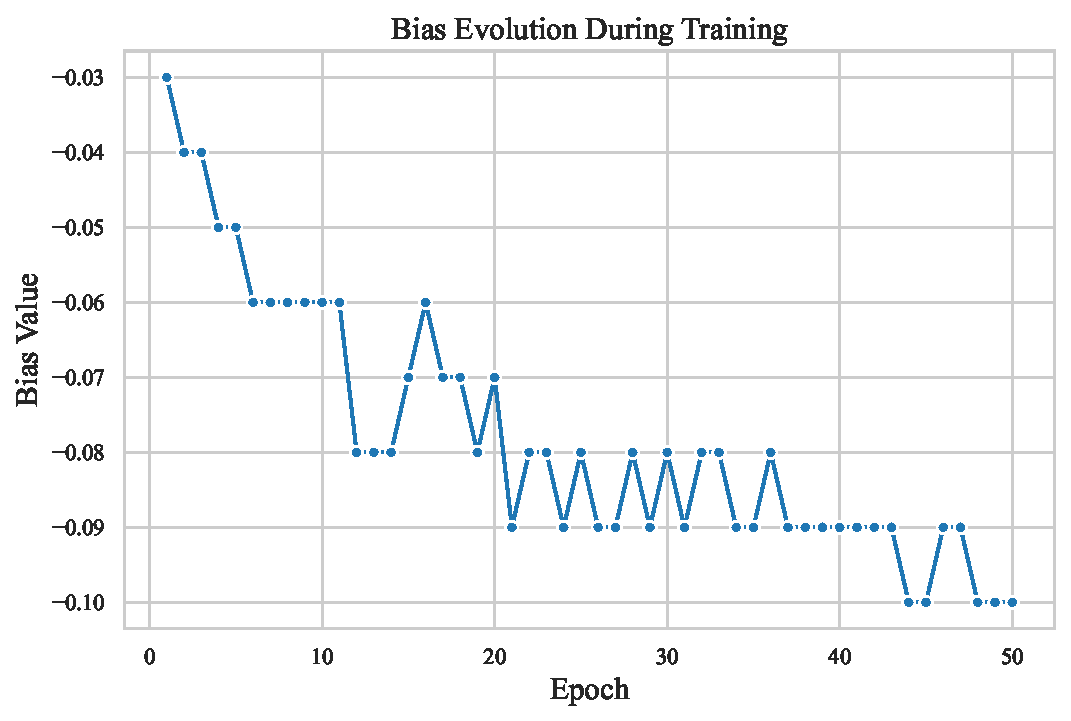
\includegraphics[width=0.6\textwidth]{bias_evolution.pdf}
\caption{Bias Evolution over Epochs}
\end{figure}
\textbf{Observation:} The bias steadily drifts more negative and settles around $-0.10$, shifting the decision boundary away from the origin to better fit the data.

\begin{figure}[H]
\centering
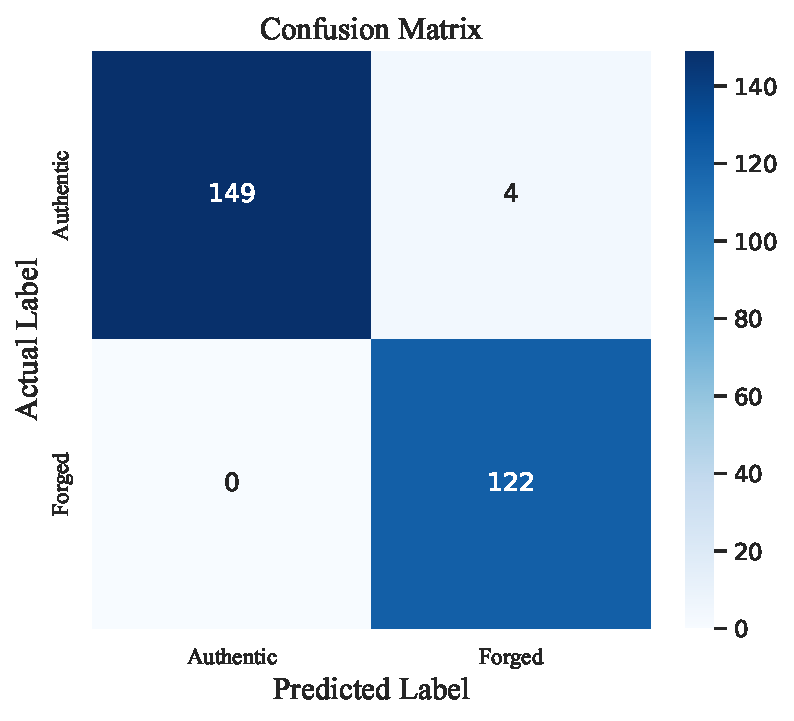
\includegraphics[width=0.5\textwidth]{confusion_matrix.pdf}
\caption{Confusion Matrix}
\end{figure}
\textbf{Observation:} 149 authentic and 122 forged notes were classified correctly, with only 4 false positives and zero false negatives -- the model never let a forged note through undetected.

\begin{figure}[H]
\centering
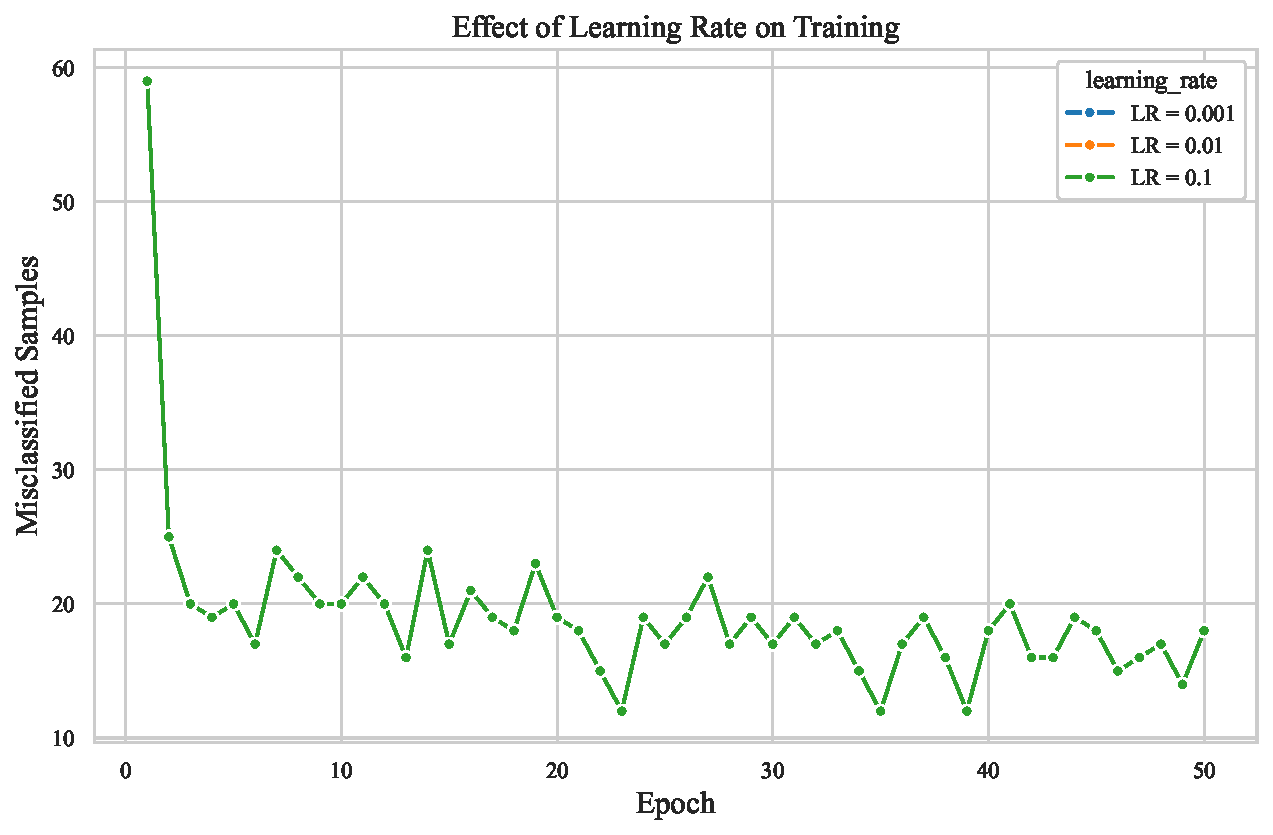
\includegraphics[width=0.6\textwidth]{learning_rate_comparison.pdf}
\caption{Learning Rate Comparison}
\end{figure}
\textbf{Observation:} All three learning rates reach the same final accuracy, but the internal error trajectory is visibly more erratic at the highest rate (0.1) and much smoother at the lowest (0.001).

\begin{figure}[H]
\centering
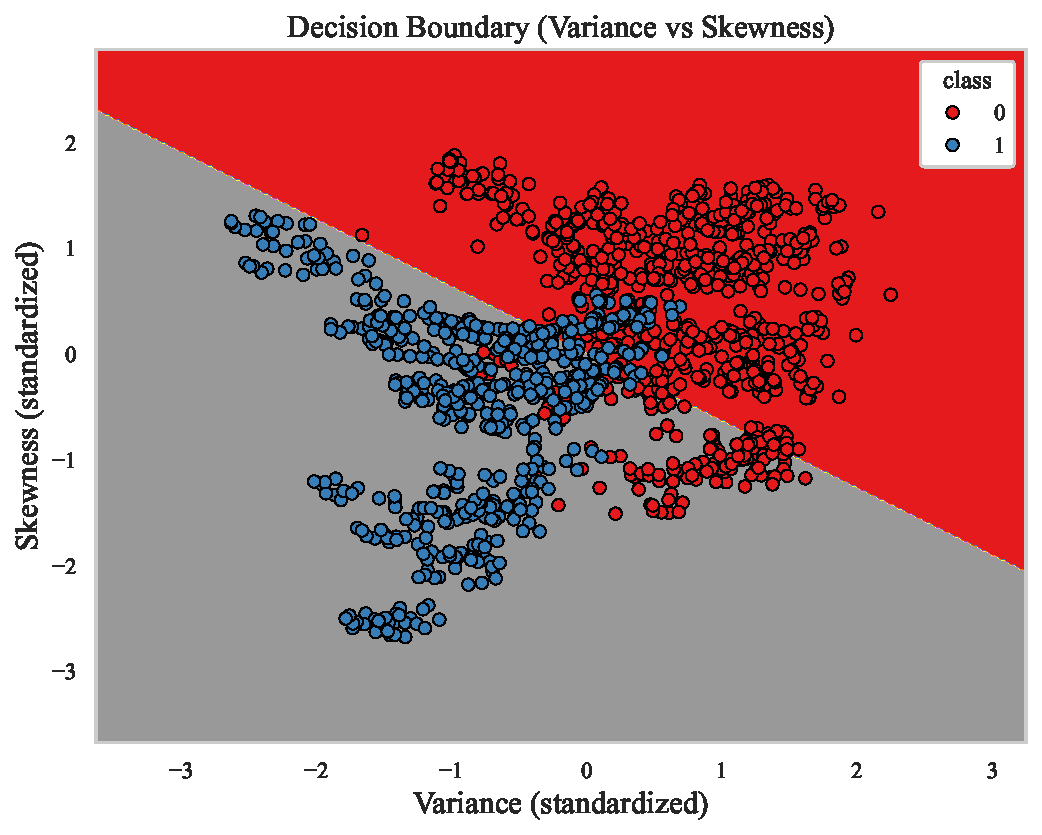
\includegraphics[width=0.6\textwidth]{decision_boundary.pdf}
\caption{Decision Boundary using Variance and Skewness}
\end{figure}
\textbf{Observation:} The 2D boundary still separates most of the two classes reasonably well, but the visible overlap region is wider than it would be with all four features available.

\begin{figure}[H]
\centering
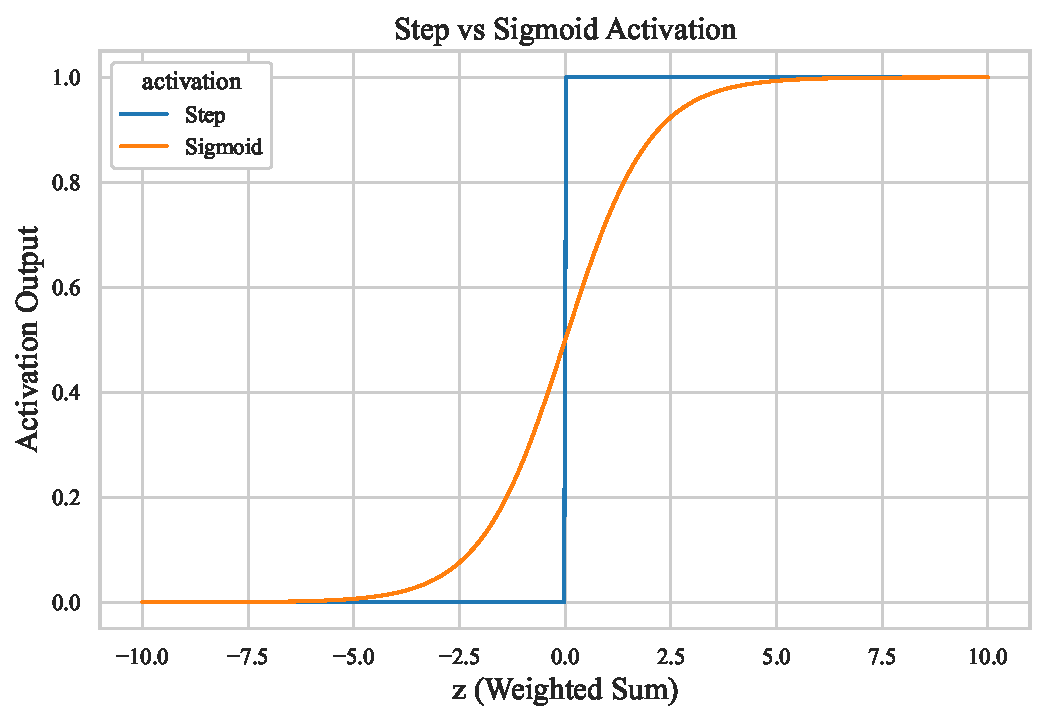
\includegraphics[width=0.6\textwidth]{step_vs_sigmoid_comparison.pdf}
\caption{Step vs. Sigmoid Activation}
\end{figure}
\textbf{Observation:} The Step function jumps sharply between 0 and 1 with no usable slope anywhere, while the Sigmoid curve is smooth and differentiable across its entire range -- exactly the property that makes gradient-based training possible.

\begin{figure}[H]
\centering
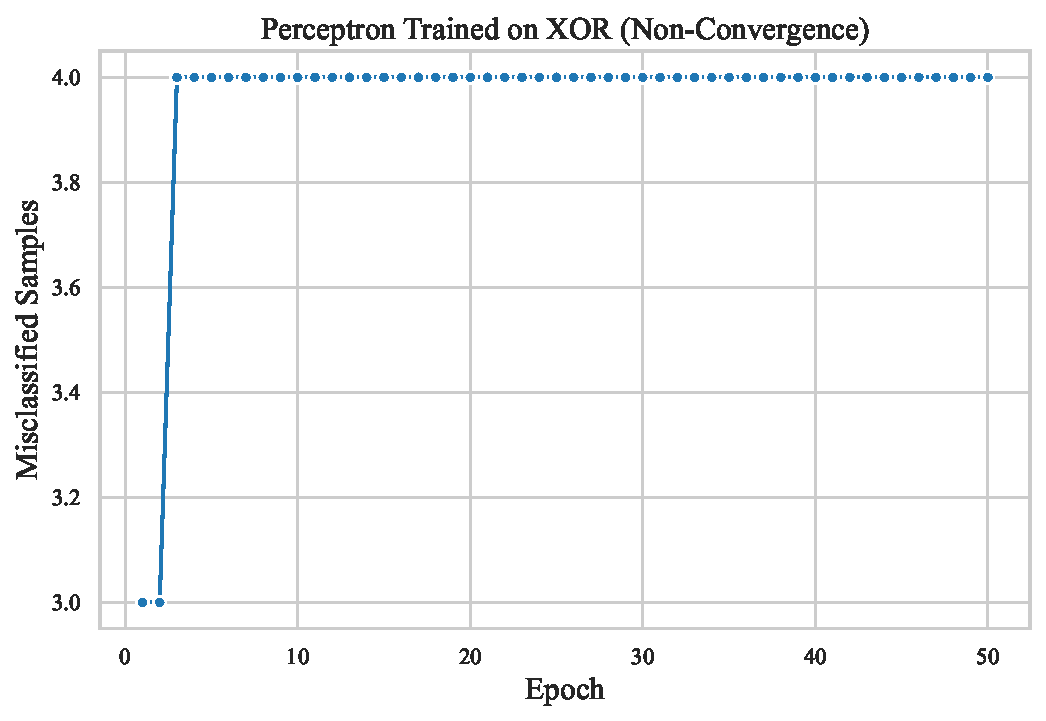
\includegraphics[width=0.6\textwidth]{xor_limitation_demo.pdf}
\caption{Perceptron Trained on XOR -- Non-Convergence}
\end{figure}
\textbf{Observation:} The error never drops to zero and stays flat near 3--4 misclassifications out of 4 points for the entire run -- direct experimental proof that a single straight-line boundary cannot solve XOR.

\begin{figure}[H]
\centering
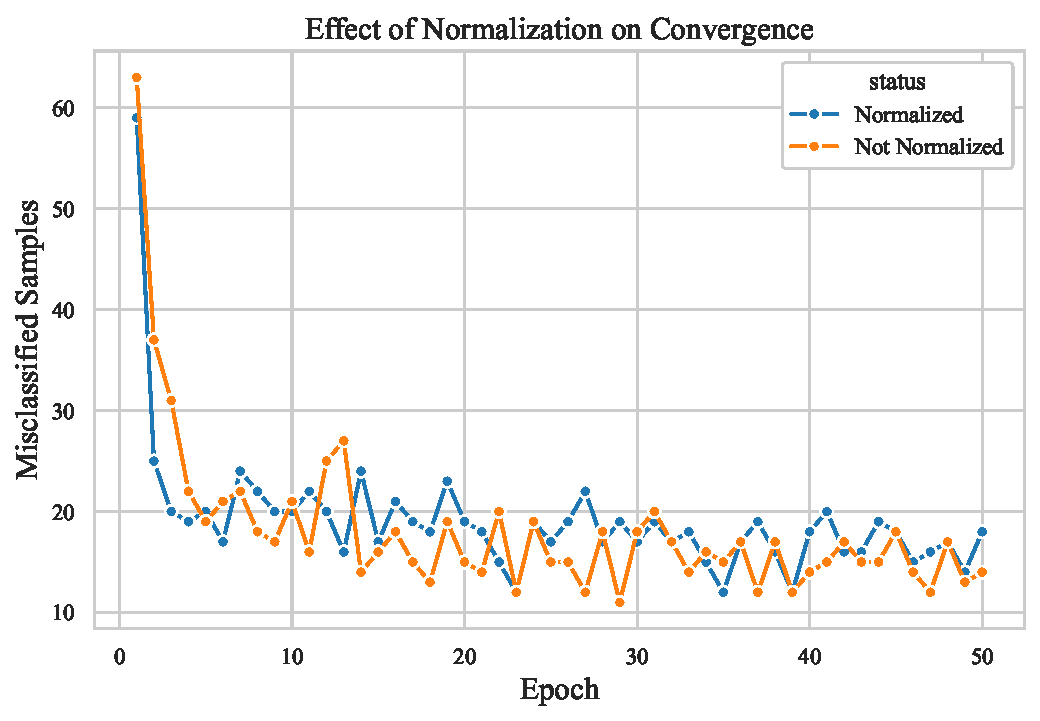
\includegraphics[width=0.6\textwidth]{normalization_effect_comparison.pdf}
\caption{Effect of Normalization on Convergence}
\end{figure}
\textbf{Observation:} The normalized run's error curve is both lower overall and noticeably smoother than the raw-feature run's curve, making the benefit of standardization clearly visible.

%----------------------------------------------------------

\section*{9. Performance Tables}

\begin{table}[H]
\centering
\caption{Training Summary}
\begin{tabular}{ll}
\toprule
Dataset Size & 1372 \\
Train/Test Split & 1097 / 275 (80\% / 20\%, stratified) \\
Learning Rate & 0.01 \\
Epochs & 50 \\
Final Weights & $[-0.1941,\ -0.2358,\ -0.2109,\ -0.0195]$ \\
Final Bias & $-0.1000$ \\
Accuracy & 0.9855 \\
Precision & 0.9683 \\
Recall & 1.0000 \\
F1-score & 0.9839 \\
\bottomrule
\end{tabular}
\end{table}

\begin{table}[H]
\centering
\caption{Epoch-wise Learning (Selected Epochs)}
\begin{tabular}{cccccc}
\toprule
Epoch & Errors & Weight 1 (Variance) & Weight 2 (Skewness) & Weight 3 (Curtosis) & Bias\\
\midrule
1  & 59 & -0.0680 & -0.0938 & -0.0678 & -0.0300 \\
5  & 20 & -0.0991 & -0.1295 & -0.1037 & -0.0500 \\
10 & 20 & -0.1307 & -0.1541 & -0.1250 & -0.0600 \\
20 & 19 & -0.1636 & -0.1946 & -0.1613 & -0.0700 \\
30 & 17 & -0.1751 & -0.2043 & -0.1901 & -0.0800 \\
40 & 18 & -0.1948 & -0.2244 & -0.1853 & -0.0900 \\
50 & 18 & -0.1941 & -0.2358 & -0.2109 & -0.1000 \\
\bottomrule
\end{tabular}
\end{table}

%----------------------------------------------------------

\section*{10. Discussion}

This experiment provides a clear, practical demonstration of how a perceptron learns, beyond the theoretical formulation alone. The model reached 98.55\% accuracy with perfect recall on the test set, consistent with the EDA pairplot, which suggested the dataset is close to linearly separable -- explaining why a simple linear model such as the perceptron performs well on it.

Several observations are worth highlighting:

\begin{itemize}[leftmargin=*]
\item The learning rate had little effect on \textit{final} accuracy in this case, but it clearly changed \textit{how} the model reached that point -- larger learning rates cause much larger, more erratic swings in the weights and bias during training.
\item Cross-checking against Scikit-learn's own Perceptron served as a useful validation step, confirming that the from-scratch implementation was not producing results by coincidence -- the two models performed almost identically.
\item Reducing the feature set to two dimensions for the decision-boundary plot noticeably degraded performance, indicating that even features with small final weights (such as Entropy) contribute meaningfully in combination with the others.
\item The XOR experiment made the linear-separability limitation directly observable rather than purely theoretical -- the error remained permanently stuck, providing concrete evidence of the boundary this class of model cannot cross.
\item The Step activation function is the central limitation of this approach: it can only express straight-line decision boundaries, provides no confidence or probability estimate, and yields no gradient signal at all. This is precisely why it is replaced by smooth, differentiable activations such as Sigmoid and ReLU in deeper, multilayer networks.
\end{itemize}

%----------------------------------------------------------

\section*{11. Conclusion}

\begin{itemize}[leftmargin=*]
\item Built a Single Layer Perceptron completely from scratch in NumPy and trained it on the real-world Banknote Authentication dataset.
\item Achieved \textbf{98.55\% accuracy}, \textbf{96.83\% precision}, \textbf{100\% recall}, and a \textbf{98.39\% F1-score} on the held-out test set.
\item Validated the implementation against Scikit-learn's Perceptron, which scored a close \textbf{97.82\% accuracy} -- confirming the from-scratch model was implemented correctly.
\item Learning rate (0.001 / 0.01 / 0.1) changed the training dynamics but not the final accuracy on this dataset.
\item Feature normalization made a real, visible difference to how smoothly and reliably the model converged.
\item Demonstrated experimentally that a single-layer perceptron cannot solve the XOR problem, since XOR is not linearly separable -- this is the exact reason Multilayer Perceptrons exist.
\item Overall, this experiment built a solid, practical foundation for the deeper architectures coming up later in this course, since every one of them is ultimately built out of these same basic ideas: weights, biases, activation functions, and gradient-based learning.
\end{itemize}

%----------------------------------------------------------

\section*{12. References}

\begin{enumerate}
\item F. Rosenblatt, ``The Perceptron,'' \emph{Psychological Review}, 1958.
\item I. Goodfellow, Y. Bengio and A. Courville, \emph{Deep Learning}, MIT Press, 2016.
\item C. M. Bishop, \emph{Pattern Recognition and Machine Learning}, Springer, 2006.
\item S. Haykin, \emph{Neural Networks and Learning Machines}, Pearson, 2009.
\item UCI Machine Learning Repository -- Banknote Authentication Dataset.
\item Scikit-learn Documentation: Perceptron.
\end{enumerate}

\end{document}